\documentclass[10pt,leqno]{article}
\usepackage[a4paper,margin=22mm,headheight=14pt]{geometry}
\usepackage{fontspec}
\setmainfont{Cambria}
\usepackage{amsmath,amssymb,amscd,mathtools}
\makeatletter
\renewcommand{\tagform@}[1]{\maketag@@@{\bfseries(#1)}}
\makeatother
\usepackage{unicode-math}
\setmathfont{Cambria Math}
\usepackage{graphicx,fancyhdr,microtype,seqsplit}
\graphicspath{{../assets/presentation_derivatives/}{./}}
\usepackage[hidelinks]{hyperref}
\setlength{\parindent}{0pt}
\setlength{\parskip}{.4em}
\setlength{\emergencystretch}{3em}
\allowdisplaybreaks
\pagestyle{fancy}\fancyhf{}
\renewcommand{\headrulewidth}{0pt}
\fancyhead[C]{\ifnum\value{page}=273\else\ifodd\value{page}LA CONJECTURE DE WEIL. I\else PIERRE DELIGNE\fi\fi}
\fancyhead[L]{\ifodd\value{page}\else\thepage\fi}
\fancyhead[R]{\ifnum\value{page}=273\else\ifodd\value{page}\thepage\fi\fi}
\fancyfoot[L]{\ifodd\value{page}\else\textit{\thepage}\fi}
\fancyfoot[R]{\ifodd\value{page}\ifnum\value{page}=273 \shortstack[r]{\textit{\thepage}\\35}\else\ifnum\value{page}=281 \shortstack[r]{\textit{\thepage}\\36}\else\textit{\thepage}\fi\fi\fi}
\usepackage{tikz}
\usetikzlibrary{calc}
\begin{document}
% ---- 01 ----
\setcounter{page}{273}


\begin{center}{\Large\bfseries THE WEIL CONJECTURE. I}\par\medskip \emph{by} \textsc{Pierre} DELIGNE\end{center}

\phantomsection\label{physical-2}

\section*{CONTENTS}

\noindent 1. Grothendieck’s theory: cohomological interpretation of \(\mathrm{L}\)-functions\dotfill 273\par

\noindent 2. Grothendieck’s theory: Poincaré duality\dotfill 280\par

\noindent 3. The fundamental estimate\dotfill 283\par

\noindent 4. Lefschetz theory: local theory\dotfill 287\par

\noindent 5. Lefschetz theory: global theory\dotfill 289\par

\noindent 6. A rationality theorem\dotfill 294\par

\noindent 7. Completion of the proof of (1.7)\dotfill 298\par

\noindent 8. First applications\dotfill 301\par

\noindent In this paper, I prove the Weil conjecture concerning the eigenvalues of Frobenius endomorphisms. A precise statement appears in (1.6). I have sought to present the proof in as geometric and elementary a form as possible and have included numerous reminders: only the results of §§ 3, 6, 7 and 8 are original.\par

\noindent In a sequel to this paper, I shall give various refinements of the intermediate results, and applications, among them the “hard” Lefschetz theorem (on iterated cup products with the cohomology class of a hyperplane section).\par

\noindent The text follows faithfully that of six lectures delivered at Cambridge in July 1973. I am grateful to \(\mathrm{N}\). Katz for permission to use his notes.\par

\section*{1. Grothendieck’s theory: cohomological interpretation of \(\mathrm{L}\)-functions.}

\noindent \textbf{(1.1)} Let \(\mathrm{X}\) be a scheme of finite type over \(\mathbf{Z}, |\mathrm{X}|\) the set of closed points of \(\mathrm{X}\) and, for \(x\in |\mathrm{X}|\), let \(\mathrm{N}(x)\) be the number of elements of the residue field \(k(x)\) of \(\mathrm{X}\) at \(x\). The Hasse-Weil zeta function of \(\mathrm{X}\) is\par

\begin{equation*}\begin{gathered}\zeta _{\mathrm{X}}(s) = \prod _{x\in |\mathrm{X}|} (1 -  \mathrm{N}(x)^{- s})^{- 1}\end{gathered}\tag{1.1.1}\end{equation*}

\noindent (this product converges absolutely for \(\mathcal{R} (s)\) sufficiently large). For \(\mathrm{X} = \operatorname{Spec}(\mathbf{Z}), \zeta _{\mathrm{X}}(s)\) is the Riemann zeta function.\par

\noindent We shall restrict attention to the case where \(\mathrm{X}\) is a scheme over a finite field \(\mathbf{F}_{q}\).\par

\clearpage

\phantomsection\label{physical-3}

\noindent For \(x\in |\mathrm{X}|\), we shall write \(q_{x}\) rather than \(\mathrm{N}(x)\). Setting \(\operatorname{deg}(x)=[k(x):\mathbf{F}_{q}]\), we have \(q_{x}=q^{\operatorname{deg}(x)}\). It is useful to introduce the variable \(t=q^{- s}\). Put\par

\begin{equation*}\begin{gathered}\mathrm{Z}(\mathrm{X}; t) = \prod _{x\in |\mathrm{X}|} (1 -  t^{\operatorname{deg}(x)})^{- 1} ;\end{gathered}\tag{1.1.2}\end{equation*}

\noindent this infinite product converges for |\(t|\) sufficiently small, and we have\par

\begin{equation*}\begin{gathered}\zeta _{\mathrm{X}}(s) = \mathrm{Z}(\mathrm{X}; q^{- s}).\end{gathered}\tag{1.1.3}\end{equation*}

\noindent \textbf{(1.2)} Dwork (On the rationality of the zeta function of an algebraic variety, \emph{Amer. J. Math.}, 82, 1960, p. 631-648) and Grothendieck ([1] and SGA 5) have proved that \(\mathrm{Z}(\mathrm{X}, t)\) is a rational function of \(t\).\par

\noindent For Grothendieck, this follows as a corollary of general results in \(\ell \)-adic cohomology (\(\ell \) denotes a prime number distinct from the characteristic \(p\) of \(\mathbf{F}_{q})\). These give a cohomological interpretation of the zeros and poles of \(\mathrm{Z}(\mathrm{X}; t)\), and a functional equation when \(\mathrm{X}\) is proper and smooth. Dwork’s methods are \(p\)-adic. When \(\mathrm{X}\) is a nonsingular hypersurface in projective space, they also gave him a cohomological interpretation of the zeros and poles, and the functional equation. They inspired the crystalline theory of Grothendieck and Berthelot, which, for \(\mathrm{X}\) proper and smooth, gives a \(p\)-adic cohomological interpretation of the zeros and poles, and the functional equation. Using ideas of Washnitzer, Lubkin constructed a variant of this theory, valid only for \(\mathrm{X}\) proper, smooth and liftable to characteristic zero (A \(p\)-adic proof of Weil’s conjectures, \emph{Ann. of Math.}, 87, 1968, p. 105-255).\par

\noindent We shall make crucial use of Grothendieck’s results, and recall them below.\par

\noindent \textbf{(1.3)} Let \(\mathrm{X}\) be an algebraic variety over an algebraically closed field \(k\) of characteristic \(p\), i.e. a separated scheme of finite type over \(k\). The case \(p=0\) is not excluded. For each prime number \(\ell \ne p\), Grothendieck defined \(\ell \)-adic cohomology groups \(\mathrm{H}^{i}(\mathrm{X}, \mathbf{Q}_{\ell })\). He also defined cohomology groups with compact support \(\mathrm{H}_{c}^{i}(\mathrm{X}, \mathbf{Q}_{\ell })\). If \(\mathrm{X}\) is proper, the two coincide. The \(\mathrm{H}_{c}^{i}(\mathrm{X}, \mathbf{Q}_{\ell })\) are finite-dimensional vector spaces over \(\mathbf{Q}_{\ell }\), vanishing for \(i>2 \operatorname{dim}(\mathrm{X})\).\par

\noindent \textbf{(1.4)} Let \(\mathrm{X}_{0}\) be an algebraic variety over \(\mathbf{F}_{q}, \overline{\mathbf{F}}_{q}\) an algebraic closure of \(\mathbf{F}_{q}\) and \(\mathrm{X}\) the algebraic variety over \(\overline{\mathbf{F}}_{q}\) obtained from \(\mathrm{X}_{0}\) by extension of scalars from \(\mathbf{F}_{q}\) to \(\overline{\mathbf{F}}_{q}\). In the terminology of Weil or Shimura, this situation would be expressed by: “Let \(\mathrm{X}\) be an algebraic variety defined over \(\mathbf{F}_{q}\)”. Let \(\mathrm{F} : \mathrm{X}\longrightarrow \mathrm{X}\) be the Frobenius morphism; it sends the point with coordinates \(x\) to the point with coordinates \(x^{q}\); in other words, if \(\mathrm{U}_{0}\) is a Zariski open subset of \(\mathrm{X}_{0}\), defining an open subset \(\mathrm{U}\) of \(\mathrm{X}\), we have \(\mathrm{F}^{- 1}(\mathrm{U})=\mathrm{U}\); for \(x\in \mathrm{H}^{0}(\mathrm{U}_{0}, \mathcal{O})\), we have \(\mathrm{F}^{*}x=x^{q}\). Let us identify the set |\(\mathrm{X}|\) of closed points of \(\mathrm{X}\) with \(\mathrm{X}_{0}(\overline{\mathbf{F}}_{q})\) (the set \(\operatorname{Hom}_{\mathbf{F}_{q}}(\operatorname{Spec}(\overline{\mathbf{F}}_{q}), \mathrm{X}_{0})\) of points of \(\mathrm{X}_{0}\) with coordinates in \(\overline{\mathbf{F}}_{q})\), and let\par

\clearpage

\phantomsection\label{physical-4}

\noindent \(\varphi \in \operatorname{Gal}(\overline{\mathbf{F}}_{q}/\mathbf{F}_{q})\) be the Frobenius substitution: \(\varphi (x)=x^{q}\). The action of \(\mathrm{F}\) on |\(\mathrm{X}|\) is identified with the action of \(\varphi \) on \(\mathrm{X}_{0}(\overline{\mathbf{F}}_{q})\). Thus:\par

\noindent \(a)\) The set \(\mathrm{X}^{\mathrm{F}}\) of closed points of \(\mathrm{X}\) fixed by \(\mathrm{F}\) is identified with the set \(\mathrm{X}_{0}(\mathbf{F}_{q})\subset \mathrm{X}_{0}(\overline{\mathbf{F}}_{q})\) of points of \(\mathrm{X}\) defined over \(\mathbf{F}_{q}\). This simply says that, for \(x\in \overline{\mathbf{F}}_{q}\), we have \(x\in \mathbf{F}_{q} \Leftrightarrow  x^{q}=x\).\par

\noindent \(b)\) Likewise, the set \(\mathrm{X}^{\mathrm{F}^{n}}\) of closed points of \(\mathrm{X}\) fixed by the \(n^{\mathrm{th}}\) iterate of \(\mathrm{F}\) is identified with \(\mathrm{X}_{0}(\mathbf{F}_{q^{n}})\).\par

\noindent \(c)\) The set |\(\mathrm{X}_{0}|\) of closed points of \(\mathrm{X}_{0}\) is identified with the set |\(\mathrm{X}|_{\mathrm{F}}\) of orbits of \(\mathrm{F}\) (or of \(\varphi )\) in |\(\mathrm{X}|\). The degree \(\operatorname{deg}(x)\) of \(x\in |\mathrm{X}_{0}|\) is the number of elements in the corresponding orbit.\par

\noindent \(d)\) From \(b)\) and \(c)\) we obtain the formula\par

\begin{equation*}\begin{gathered}\# \mathrm{X}^{\mathrm{F}^{n}} = \# \mathrm{X}_{0}(\mathbf{F}_{q^{n}}) = \sum _{\operatorname{deg}(x)|n} \operatorname{deg} x\end{gathered}\tag{1.4.1}\end{equation*}

\noindent (for \(x\in |\mathrm{X}_{0}|\) and \(\operatorname{deg}(x)|n, x\) defines \(\operatorname{deg}(x)\) points with coordinates in \(\mathbf{F}_{q^{n}}\), all conjugate over \(\mathbf{F}_{q})\).\par

\noindent \textbf{(1.5)} The morphism \(\mathrm{F}\) is finite, and in particular proper. It therefore induces maps\par

\begin{equation*}\begin{gathered}\mathrm{F}^{*} : \mathrm{H}_{c}^{i}(\mathrm{X}, \mathbf{Q}_{\ell }) \longrightarrow  \mathrm{H}_{c}^{i}(\mathrm{X}, \mathbf{Q}_{\ell }).\end{gathered}\end{equation*}

\noindent Grothendieck established the Lefschetz formula\par

\begin{equation*}\begin{gathered}\# \mathrm{X}^{\mathrm{F}} = \sum _{i} (- 1)^{i} \operatorname{Tr}(\mathrm{F}^{*}, \mathrm{H}_{c}^{i}(\mathrm{X}, \mathbf{Q}_{\ell }));\end{gathered}\end{equation*}

\noindent the right-hand side, \emph{a priori} an \(\ell \)-adic number, is an integer, and equals the left-hand side. Note that such a formula is reasonable only because \(d\mathrm{F}=0\), even at infinity (\(\mathrm{X}\) is not assumed proper); the relation \(d\mathrm{F}=0\) implies that the fixed points of \(\mathrm{F}\) have multiplicity one.\par

\noindent An analogous formula holds for the iterates of \(\mathrm{F}\):\par

\begin{equation*}\begin{gathered}\# \mathrm{X}^{\mathrm{F}^{n}} = \# \mathrm{X}_{0}(\mathbf{F}_{q^{n}}) = \sum _{i} (- 1)^{i} \operatorname{Tr}(\mathrm{F}^{*n}, \mathrm{H}_{c}^{i}(\mathrm{X}, \mathbf{Q}_{\ell })).\end{gathered}\tag{1.5.1}\end{equation*}

\noindent Let us take the logarithmic derivative of (1.1.2):\par

\begin{equation*}\begin{aligned}
t\frac{d}{dt}\log\mathrm Z(\mathrm X_0,t)&=\frac{t\frac{d}{dt}\mathrm Z(\mathrm X_0,t)}{\mathrm Z(\mathrm X_0,t)}
=\sum_{x\in|\mathrm X_0|}-\frac{-\deg(x)t^{\deg(x)}}{1-t^{\deg(x)}}\\
&=\sum_{x\in|\mathrm X_0|}\sum_{n>0}\deg(x)t^{n\cdot\deg(x)}
\underset{(1.4.1)}{=}\sum_n\#\mathrm X_0(\mathbf F_{q^n})\cdot t^n.
\end{aligned}\tag{1.5.2}\end{equation*}

\noindent For \(\mathrm{F}\) an endomorphism of a vector space \(\mathrm{V}\), we have an identity of formal series\par

\begin{equation*}\begin{gathered}t \frac{d}{dt} \operatorname{log}(\operatorname{det}(1- \mathrm{F}t, \mathrm{V})^{- 1}) = \sum _{n>0} \operatorname{Tr}(\mathrm{F}^{n}, \mathrm{V})t^{n}\end{gathered}\tag{1.5.3}\end{equation*}

\clearpage

\phantomsection\label{physical-5}

\noindent (verify this when \(\operatorname{dim}(\mathrm{V})=1\), and observe that both sides are additive in \(\mathrm{V}\) in a short exact sequence). Substituting (1.5.1) into (1.5.2) and applying (1.5.3), we find\par

\begin{equation*}\begin{gathered}t \frac{d}{dt} \operatorname{log} \mathrm{Z}(\mathrm{X}_{0},t) \\ = \sum _{i} (- 1)^{i} t \frac{d}{dt} \operatorname{log} \operatorname{det}(1- \mathrm{F}^{*}t, \mathrm{H}_{c}^{i}(\mathrm{X},\mathbf{Q}_{\ell }))^{- 1},\end{gathered}\end{equation*}

\noindent that is\par

\begin{equation*}\begin{gathered}\mathrm{Z}(\mathrm{X}_{0},t) = \prod _{i} \operatorname{det}(1- \mathrm{F}^{*}t, \mathrm{H}_{c}^{i}(\mathrm{X},\mathbf{Q}_{\ell }))^{(- 1)^{i+1}}.\end{gathered}\tag{1.5.4}\end{equation*}

\noindent The right-hand side is an element of \(\mathbf{Q}_{\ell }(t)\). The formula asserts that its Taylor expansion at \(t=0\), \emph{a priori} a formal series in \(\mathbf{Q}_{\ell }[[t]]\) with constant term one, belongs to \(\mathbf{Z}[[t]]\), and equals the left-hand side, also regarded as a formal series in \(t\). This formula gives Grothendieck’s cohomological interpretation of the function \(\mathrm{Z}\).\par

\noindent Our main result is the following.\par

\noindent \emph{Theorem} \textbf{(1.6)}. — {\itshape Let \(\mathrm{X}_{0}\) be a nonsingular (= smooth) projective variety over \(\mathbf{F}_{q}\). For each \(i\), the characteristic polynomial \(\operatorname{det}(t\cdot 1- \mathrm{F}^{*}, \mathrm{H}^{i}(\mathrm{X},\mathbf{Q}_{\ell }))\) has integer coefficients independent of \(\ell  (\ell \ne p)\). The complex roots \(\alpha \) of this polynomial (the complex conjugates of the eigenvalues of \(\mathrm{F}^{*})\) have absolute value |\(\alpha |=q^{i/2}\).}\par

\noindent Let us first show that (1.6) follows from the following apparently weaker result.\par

\noindent \emph{Lemma} \textbf{(1.7)}. — {\itshape For each \(i\), and each \(\ell \ne p\), the eigenvalues of the endomorphism \(\mathrm{F}^{*}\) of \(\mathrm{H}^{i}(\mathrm{X},\mathbf{Q}_{\ell })\) are algebraic numbers all of whose complex conjugates \(\alpha \) have absolute value |\(\alpha |=q^{i/2}\).}\par

\noindent \emph{Proof of} (\(1.7) \Rightarrow  (1.6)\). — Regard \(\mathrm{Z}(\mathrm{X}_{0},t)\) as a formal series with constant term 1, an element of \(\mathbf{Z}[[t]] : \mathrm{Z}(\mathrm{X}_{0},t)=\sum _{n} a_{n} t^{n}\). By (1.5.4), the image of \(\mathrm{Z}(\mathrm{X}_{0},t)\) in \(\mathbf{Q}_{\ell }[[t]]\) is the Taylor expansion of a rational function. This means that for \(\mathrm{N}\) and \(\mathrm{M}\) sufficiently large (\(\geq \) the degrees of the numerators and denominators) the Hankel determinants\par

\begin{equation*}\begin{gathered}\mathrm{H}_{k} = \operatorname{det}((a_{i+j+k})_{0\leq i,j\leq \mathrm{M}})    (k>\mathrm{N})\end{gathered}\end{equation*}

\noindent vanish. This vanishing holds in \(\mathbf{Q}_{\ell }\) if and only if it holds in \(\mathbf{Q}; \mathrm{Z}(\mathrm{X}_{0},t)\) is therefore the Taylor series expansion of an element of \(\mathbf{Q}(t)\). In other words,\par

\begin{equation*}\begin{gathered}\mathrm{Z}(\mathrm{X}_{0},t) \in  \mathbf{Z}[[t]] \cap  \mathbf{Q}_{\ell }(t) \subset  \mathbf{Q}(t).\end{gathered}\end{equation*}

\noindent Write \(\mathrm{Z}(\mathrm{X}_{0},t)=\mathrm{P}/\mathrm{Q}\), with \(\mathrm{P},\mathrm{Q}\in \mathbf{Z}[t]\), relatively prime, and with positive constant terms. By a lemma of Fatou, the fact that \(\mathrm{Z}(\mathrm{X}_{0},t)\) belongs to \(\mathbf{Z}[[t]]\) and has constant term one implies that the constant terms of \(\mathrm{P}\) and \(\mathrm{Q}\) are 1. Put\par

\begin{equation*}\begin{gathered}\mathrm{P}_{i}(t)=\operatorname{det}(1- \mathrm{F}^{*}t, \mathrm{H}^{i}(\mathrm{X},\mathbf{Q}_{\ell })).\end{gathered}\end{equation*}

\clearpage

\phantomsection\label{physical-6}

\noindent Under hypothesis (1.7), the \(\mathrm{P}_{i}\) are pairwise relatively prime. The right-hand side of (1.5.4) is therefore in reduced form, and\par

\begin{equation*}\begin{gathered}\mathrm{P}(t) = \prod _{i \text{odd}} \mathrm{P}_{i}(t) \\ \mathrm{Q}(t) = \prod _{i \text{even}} \mathrm{P}_{i}(t).\end{gathered}\end{equation*}

\noindent Let \(\mathrm{K}\) be the subfield of an algebraic closure \(\overline{\mathbf{Q}}_{\ell }\) of \(\mathbf{Q}_{\ell }\) generated over \(\mathbf{Q}\) by the roots of \(\mathrm{R}(t)=\mathrm{P}(t)\mathrm{Q}(t)\). The roots of \(\mathrm{P}_{i}(t)\) are those roots of \(\mathrm{R}(t)\) with the property that all their complex conjugates have absolute value \(q^{- i/2}\). This set is stable under \(\operatorname{Gal}(\mathrm{K}/\mathbf{Q})\). Hence the polynomial \(\mathrm{P}_{i}(t)\) has rational coefficients. By Gauss’s lemma (or because the roots of \(\mathrm{P}_{i}\), being roots of \(\mathrm{R}(t)\), are reciprocals of algebraic integers), it even has integer coefficients. The above description of the roots of \(\mathrm{P}_{i}(t)\) is independent of \(\ell \); the polynomial \(\mathrm{P}_{i}(t)\) itself is therefore independent of \(\ell \).\par

\noindent The remainder of this paper is devoted to the proof of (1.7).\par

\noindent \textbf{(1.8)} Grothendieck’s theory supplies a cohomological interpretation not only of zeta functions, but also of \(\mathrm{L}\)-functions. Here are the results.\par

\noindent \textbf{(1.9)} Let \(\mathrm{X}\) be an algebraic variety over a field \(k\). For the definition of a constructible \(\mathbf{Q}_{\ell }\)-sheaf on \(\mathrm{X}\), I refer to SGA 5 VI. It suffices to say that:\par

\noindent \(a)\) If \(\mathcal{F} \) is a constructible \(\mathbf{Q}_{\ell }\)-sheaf on \(\mathrm{X}\), there is a finite partition of \(\mathrm{X}\) into locally closed subsets \(\mathrm{X}_{i}\) such that \(\mathcal{F} |\mathrm{X}_{i}\) is locally constant.\par

\noindent \(b)\) Assume that \(\mathrm{X}\) is connected and let \(\overline{x}\) be a geometric point of \(\mathrm{X}\). When \(\mathcal{F} \) is locally constant, \(\pi _{1}(\mathrm{X},\overline{x})\) acts on the fiber \(\mathcal{F} _{\overline{x}}\); the fiber functor at \(\overline{x}\) is an equivalence of categories\par

\begin{center}(constructible locally constant \(\mathbf{Q}_{\ell }\)-sheaves on \(\mathrm{X}) \longmapsto \)\\ \(\longmapsto \) (continuous representations of \(\pi _{1}(\mathrm{X},\overline{x})\) on a finite-dimensional \(\mathbf{Q}_{\ell }\)-vector space).\end{center}

\noindent A representation of this kind does not, in general, factor through a finite quotient of \(\pi _{1}(\mathrm{X},\overline{x})\).\par

\noindent \(c)\) If \(k=\mathbf{C}\), constructible \(\mathbf{Q}_{\ell }\)-sheaves on \(\mathrm{X}\) are identified with sheaves of \(\mathbf{Q}_{\ell }\)-vector spaces \(\mathcal{F} \) on \(\mathrm{X}^{\mathrm{an}}\), for which there is a finite partition of \(\mathrm{X}\) into Zariski-locally closed subsets \(\mathrm{X}_{i}\), and for each \(i\) a local system of finite free \(\mathbf{Z}_{\ell }\)-Modules \(\mathcal{F} _{i}\) on \(\mathrm{X}_{i}\), with\par

\begin{equation*}\begin{gathered}\mathcal{F} |\mathrm{X}_{i} = \mathcal{F} _{i} \otimes _{\mathbf{Z}_{\ell }} \mathbf{Q}_{\ell }.\end{gathered}\end{equation*}

\noindent We shall consider only constructible \(\mathbf{Q}_{\ell }\)-sheaves, and shall call them simply \(\mathbf{Q}_{\ell }\)-sheaves.\par

\noindent \textbf{(1.10)} Assume that \(k\) is algebraically closed, and let \(\mathcal{F} \) be a \(\mathbf{Q}_{\ell }\)-sheaf on \(\mathrm{X}\). Grothendieck defined \(\ell \)-adic cohomology groups \(\mathrm{H}^{i}(\mathrm{X},\mathcal{F} )\) and \(\mathrm{H}_{c}^{i}(\mathrm{X},\mathcal{F} )\). The \(\mathrm{H}_{c}^{i}(\mathrm{X},\mathcal{F} )\) are finite-dimensional vector spaces over \(\mathbf{Q}_{\ell }\), vanishing for \(i>2 \operatorname{dim}(\mathrm{X})\).\par

\clearpage

\phantomsection\label{physical-7}

\noindent For \(k=\mathbf{C}\), the \(\mathrm{H}^{i}(\mathrm{X},\mathcal{F} )\) and \(\mathrm{H}_{c}^{i}(\mathrm{X},\mathcal{F} )\) are the usual cohomology groups (respectively, with compact support) of \(\mathrm{X}^{\mathrm{an}}\), with coefficients in \(\mathcal{F} \).\par

\noindent \textbf{(1.11)} Let \(\mathrm{X}_{0}\) be an algebraic variety over \(\mathbf{F}_{q}, \mathrm{X}\) the corresponding variety over \(\overline{\mathbf{F}}_{q}\), and \(\mathcal{F} _{0}\) a sheaf of sets on \(\mathrm{X}_{0}\) (for the étale topology). Write \(\mathcal{F} \) for its inverse image on \(\mathrm{X}\). Besides the Frobenius morphism \(\mathrm{F} : \mathrm{X}\longrightarrow \mathrm{X}\), we then have a canonical isomorphism \(\mathrm{F}^{*} : \mathrm{F}^{*}\mathcal{F}  \xrightarrow{\sim } \mathcal{F} \). Here is a description of it. View \(\mathcal{F} _{0}\) as an étalé space over \(\mathrm{X}_{0}\), i.e. identify \(\mathcal{F} _{0}\) with the algebraic space [\(\mathcal{F} _{0}]\), equipped with an étale morphism \(f : [\mathcal{F} _{0}]\longrightarrow \mathrm{X}_{0}\), such that \(\mathcal{F} _{0}\) is the sheaf of local sections of [\(\mathcal{F} _{0}]\). The analogous space [\(\mathcal{F} ]\), étalé over \(\mathrm{X}\), is obtained from [\(\mathcal{F} _{0}]\) by extension of scalars. We thus have a commutative diagram\par

\[\begin{array}{ccc}[\mathcal F]&\xrightarrow{\mathrm F}&[\mathcal F]\\ \downarrow\!f&&\downarrow\!f\\ \mathrm X&\xrightarrow{\mathrm F}&\mathrm X\end{array}\]

\noindent hence a morphism [\(\mathcal{F} ]\longrightarrow \mathrm{X}\times _{(\mathrm{F},\mathrm{X},f)}[\mathcal{F} ]=[\mathrm{F}^{*}\mathcal{F} ]\), which is an isomorphism since \(f\) is étale. Its inverse gives the desired isomorphism \(\mathrm{F}^{*}\mathcal{F}  \xrightarrow{\sim } \mathcal{F} \).\par

\noindent This construction extends to \(\mathbf{Q}_{\ell }\)-sheaves.\par

\noindent \textbf{(1.12)} Let \(\mathrm{X}_{0}\) be an algebraic variety over \(\mathbf{F}_{q}, \mathcal{F} _{0}\) a \(\mathbf{Q}_{\ell }\)-sheaf on \(\mathrm{X}_{0}, (\mathrm{X},\mathcal{F} )\) obtained from (\(\mathrm{X}_{0},\mathcal{F} _{0})\) by extension of scalars from \(\mathbf{F}_{q}\) to \(\overline{\mathbf{F}}_{q}, \mathrm{F} : \mathrm{X}\longrightarrow \mathrm{X}\) and \(\mathrm{F}^{*} : \mathrm{F}^{*}\mathcal{F} \longrightarrow \mathcal{F} \).\par

\noindent The finite morphism \(\mathrm{F}\), together with \(\mathrm{F}^{*}\), defines an endomorphism\par

\begin{equation*}\begin{gathered}\mathrm{F}^{*} : \mathrm{H}_{c}^{i}(\mathrm{X},\mathcal{F} ) \longrightarrow  \mathrm{H}_{c}^{i}(\mathrm{X},\mathrm{F}^{*}\mathcal{F} ) \longrightarrow  \mathrm{H}_{c}^{i}(\mathrm{X},\mathcal{F} ).\end{gathered}\end{equation*}

\noindent For \(x\in |\mathrm{X}|, \mathrm{F}^{*}\) defines a morphism \(\mathrm{F}_{x}^{*} : \mathcal{F} _{\mathrm{F}(x)}\longrightarrow \mathcal{F} _{x}\). For \(x\in \mathrm{X}^{\mathrm{F}}\), this is an endomorphism of \(\mathcal{F} _{x}\). Grothendieck proved the Lefschetz formula\par

\begin{equation*}\begin{gathered}\sum _{x\in \mathrm{X}^{\mathrm{F}}} \operatorname{Tr}(\mathrm{F}_{x}^{*},\mathcal{F} _{x}) = \sum _{i} (- 1)^{i} \operatorname{Tr}(\mathrm{F}^{*},\mathrm{H}_{c}^{i}(\mathrm{X},\mathcal{F} )).\end{gathered}\end{equation*}

\noindent An analogous formula holds for the iterates of \(\mathrm{F}\): the \(n^{\mathrm{th}}\) iterate of \(\mathrm{F}^{*}\) defines morphisms \(\mathrm{F}_{x}^{*n} : \mathcal{F} _{\mathrm{F}_{x}^{n}(x)}\longrightarrow \mathcal{F} _{x}\); for \(x\) fixed by \(\mathrm{F}^{n}, \mathrm{F}_{x}^{*n}\) is an endomorphism, and\par

\begin{equation*}\begin{gathered}\sum _{x\in \mathrm{X}^{\mathrm{F}^{n}}} \operatorname{Tr}(\mathrm{F}_{x}^{*n},\mathcal{F} _{x}) = \sum _{i} (- 1)^{i} \operatorname{Tr}(\mathrm{F}^{*n},\mathrm{H}_{c}^{i}(\mathrm{X},\mathcal{F} )).\end{gathered}\tag{1.12.1}\end{equation*}

\noindent \textbf{(1.13)} Let \(x_{0}\in |\mathrm{X}_{0}|, \mathrm{Z}\) be the corresponding orbit of \(\mathrm{F}\) in |\(\mathrm{X}|\) and \(x\in \mathrm{Z}\). The orbit \(\mathrm{Z}\) has \(\operatorname{deg}(x_{0})\) elements (1.4). Write \(\mathrm{F}_{x_{0}}^{*}\) for the endomorphism \(\mathrm{F}_{x}^{*\operatorname{deg}(x_{0})}\) of \(\mathcal{F} _{x}\), and put\par

\begin{equation*}\begin{gathered}\operatorname{det}(1- \mathrm{F}_{x_{0}}^{*}t,\mathcal{F} _{0}) = \operatorname{det}(1- \mathrm{F}_{x_{0}}^{*}t,\mathcal{F} _{x}).\end{gathered}\end{equation*}

\noindent Up to isomorphism, (\(\mathcal{F} _{x},\mathrm{F}_{x_{0}}^{*})\) is independent of the choice of \(x\). This justifies leaving \(x\) out of the notation. Similar notation will be used for other functions of (\(\mathcal{F} _{x},\mathrm{F}_{x_{0}}^{*})\).\par

\clearpage

\phantomsection\label{physical-8}

\noindent \textbf{(1.14)} Define \(\mathrm{Z}(\mathrm{X}_{0},\mathcal{F} _{0},t)\in \mathbf{Q}_{\ell }[[t]]\) by the product\par

\begin{equation*}\begin{gathered}\mathrm{Z}(\mathrm{X}_{0},\mathcal{F} _{0},t) = \prod _{x\in |\mathrm{X}_{0}|} \operatorname{det}(1- \mathrm{F}_{x}^{*}t^{\operatorname{deg}(x)},\mathcal{F} _{0})^{- 1}.\end{gathered}\tag{1.14.1}\end{equation*}

\noindent When \(\mathcal{F} \) is the constant sheaf \(\mathbf{Q}_{\ell }\), we recover (1.1.2). Formula (1.5.3) gives the logarithmic derivative of \(\mathrm{Z}\) as\par

\begin{equation*}\begin{aligned}
t\frac{d}{dt}\log\mathrm Z(\mathrm X_0,\mathcal F_0,t)
&\underset{\mathrm{dfn}}{=}\frac{t\frac{d}{dt}\mathrm Z(\mathrm X_0,\mathcal F_0,t)}{\mathrm Z(\mathrm X_0,\mathcal F_0,t)}\\
&=\sum_n\sum_{x\in\mathrm X^{\mathrm F^n}=\mathrm X_0(\mathbf F_{q^n})}\operatorname{Tr}(\mathrm F_x^{*n},\mathcal F_0)t^n.
\end{aligned}\tag{1.14.2}\end{equation*}

\noindent Substituting (1.12.1) into (1.14.2), we obtain, by the same calculation as in (1.5), the following generalization of (1.5.4)\par

\begin{equation*}\begin{gathered}\mathrm{Z}(\mathrm{X}_{0},\mathcal{F} _{0},t) = \prod _{i} \operatorname{det}(1- \mathrm{F}^{*}t,\mathrm{H}_{c}^{i}(\mathrm{X},\mathcal{F} ))^{(- 1)^{i+1}}.\end{gathered}\tag{1.14.3}\end{equation*}

\noindent This formula is an identity in \(\mathbf{Q}_{\ell }[[t]]\).\par

\noindent \textbf{(1.15)} It is sometimes useful to employ Galois-theoretic rather than geometric language. Here is the dictionary.\par

\noindent If \(\overline{\mathbf{F}}_{q}^{1}\) and \(\overline{\mathbf{F}}_{q}^{2}\) are two algebraic closures of \(\mathbf{F}_{q}, (\mathrm{X}_{0},\mathcal{F} _{0})\) over \(\mathbf{F}_{q}\) defines, by extension of scalars, (\(\mathrm{X}_{1},\mathcal{F} _{1})\) over \(\overline{\mathbf{F}}_{q}^{1}\) and (\(\mathrm{X}_{2},\mathcal{F} _{2})\) over \(\overline{\mathbf{F}}_{q}^{2}\). Any \(\mathbf{F}_{q}\)-isomorphism \(\sigma  : \overline{\mathbf{F}}_{q}^{1} \xrightarrow{\sim } \overline{\mathbf{F}}_{q}^{2}\) induces an isomorphism\par

\begin{equation*}\begin{gathered}\mathrm{H}_{c}^{*}(\mathrm{X}_{1},\mathcal{F} _{1}) \xrightarrow{\sim } \mathrm{H}_{c}^{*}(\mathrm{X}_{2},\mathcal{F} _{2}).\end{gathered}\end{equation*}

\noindent In particular, when \(\overline{\mathbf{F}}_{q}^{1}=\overline{\mathbf{F}}_{q}^{2}\) (denoted \(\overline{\mathbf{F}}_{q})\), we find that \(\operatorname{Gal}(\overline{\mathbf{F}}_{q}/\mathbf{F}_{q})\) acts on \(\mathrm{H}_{c}^{*}(\mathrm{X},\mathcal{F} )\) (action by transport of structure). Let \(\varphi \in \operatorname{Gal}(\overline{\mathbf{F}}_{q}/\mathbf{F}_{q})\) be the Frobenius substitution. One checks that\par

\begin{equation*}\begin{gathered}\mathrm{F}^{*} = \varphi ^{- 1}    (\text{ in }\operatorname{End}(\mathrm{H}_{c}^{*}(\mathrm{X},\mathcal{F} ))).\end{gathered}\end{equation*}

\noindent This leads to defining the \emph{geometric Frobenius} \(\mathrm{F}\in \operatorname{Gal}(\overline{\mathbf{F}}_{q}/\mathbf{F}_{q})\) to be \(\varphi ^{- 1}\). We have\par

\begin{equation*}\begin{gathered}\mathrm{F}^{*} = \mathrm{F}.\end{gathered}\tag{1.15.1}\end{equation*}

\noindent Let \(x\) be a geometric point of \(\mathrm{X}_{0}\), lying over \(x_{0}\in |\mathrm{X}_{0}|\). By transport of structure, the group \(\operatorname{Gal}(k(x)/k(x_{0}))\) acts on the fiber (\(\mathcal{F} _{0})_{x}\) of \(\mathcal{F} _{0}\) at \(x\); in particular, the geometric Frobenius relative to \(k(x_{0}) : \mathrm{F}_{x_{0}}\in \operatorname{Gal}(k(x)/k(x_{0}))\) acts. For \(x\) defined by a closed point, again denoted \(x\), of \(\mathrm{X}\), we have \(\mathcal{F} _{x}=(\mathcal{F} _{0})_{x}\), and\par

\begin{equation*}\begin{gathered}\mathrm{F}_{x_{0}}^{*} \underset{\mathrm{dfn}}{=} \mathrm{F}_{x}^{*\operatorname{deg}(x_{0})} = \mathrm{F}_{x_{0}}    (\text{ in }\operatorname{End}(\mathcal{F} _{x})).\end{gathered}\tag{1.15.2}\end{equation*}

\noindent In Galois notation, (1.14.3) becomes\par

\begin{equation*}\begin{gathered}\prod _{x\in |\mathrm{X}_{0}|} \operatorname{det}(1- \mathrm{F}_{x} t^{\operatorname{deg}(x)},\mathcal{F} _{0})^{- 1} \\ = \prod _{i} \operatorname{det}(1- \mathrm{F}t,\mathrm{H}_{c}^{i}(\mathrm{X},\mathcal{F} ))^{(- 1)^{i+1}}.\end{gathered}\end{equation*}

\clearpage

\phantomsection\label{physical-9}

\section*{2. Grothendieck’s theory: Poincaré duality.}

\noindent \textbf{(2.1)} To explain the relation between roots of unity and orientations, I shall first recast two classical cases in fanciful language.\par

\noindent a) \emph{Differentiable manifolds}. — Let \(\mathrm{X}\) be a differentiable manifold of pure dimension \(n\). The orientation sheaf \(\mathbf{Z}'\) on \(\mathrm{X}\) is the sheaf locally isomorphic to the constant sheaf \(\mathbf{Z}\), whose invertible sections over an open subset \(\mathrm{U}\) of \(\mathrm{X}\) correspond to orientations of \(\mathrm{U}\). An \emph{orientation} of \(\mathrm{X}\) is an isomorphism from \(\mathbf{Z}'\) to the constant sheaf \(\mathbf{Z}\). The \emph{fundamental class} of \(\mathrm{X}\) is a morphism \(\operatorname{Tr} : \mathrm{H}_{c}^{n}(\mathrm{X},\mathbf{Z}')\longrightarrow \mathbf{Z}\); if \(\mathrm{X}\) is oriented, it is identified with a morphism \(\operatorname{Tr} : \mathrm{H}_{c}^{n}(\mathrm{X},\mathbf{Z})\longrightarrow \mathbf{Z}\). Poincaré duality is expressed in terms of the fundamental class.\par

\noindent b) \emph{Complex varieties}. — Let \(\mathbf{C}\) be an algebraic closure of \(\mathbf{R}\). A smooth complex algebraic variety, or rather its underlying differentiable manifold, is always orientable. Orienting \(\mathbf{C}\) itself suffices to orient it. Equivalently, one may:\par

\noindent \(a)\) choose one of the two roots of the equation \(\mathrm{X}^{2}=- 1\); call it +\(i\);\par

\noindent \(b)\) choose an isomorphism of \(\mathbf{R}/\mathbf{Z}\) with \(\mathrm{U}^{1}=\{z\in \mathbf{C} | |z|=1\}; +i\) is the image of \(1/4\);\par

\noindent \(c)\) choose one of the two isomorphisms \(x\longmapsto \operatorname{exp}(\pm 2\pi ix)\) from \(\mathbf{Q}/\mathbf{Z}\) onto the group of roots of unity in \(\mathbf{C}\), which extends continuously to an isomorphism from \(\mathbf{R}/\mathbf{Z}\) onto \(\mathrm{U}^{1}\).\par

\noindent Write \(\mathbf{Z}(1)\) for a free \(\mathbf{Z}\)-module of rank one whose two-element set of generators is in canonical correspondence with one of the two-element sets \(a)\), \(b), c)\). The simplest choice is to take \(\mathbf{Z}(1)=\operatorname{Ker}(\operatorname{exp} : \mathbf{C}\longrightarrow \mathbf{C}^{*})\). The generator \(y=\pm 2\pi i\) corresponds to the isomorphism \(c) : x\longmapsto \operatorname{exp}(xy)\).\par

\noindent Let \(\mathbf{Z}(r)\) be the \(r^{\mathrm{th}}\) tensor power of \(\mathbf{Z}(1)\). If \(\mathrm{X}\) is a smooth complex algebraic variety of pure complex dimension \(r\), the orientation sheaf of \(\mathrm{X}\) is the constant sheaf with value \(\mathbf{Z}(r)\).\par

\noindent \textbf{(2.2)} To “orient” algebraic varieties over an algebraically closed field \(k\) of characteristic 0, one must choose an isomorphism from \(\mathbf{Q}/\mathbf{Z}\) onto the group of roots of unity in \(k\). The set of these isomorphisms is a principal homogeneous space under \(\widehat{\mathbf{Z}}^{*}\) (no longer under \(\mathbf{Z}^{*})\). If only \(\ell \)-adic cohomology is of interest, it suffices to consider roots of unity whose order is a power of \(\ell \), and to assume that the characteristic \(p\) of \(k\) is distinct from \(\ell \). Write \(\mathbf{Z}/\ell ^{n}(1)\) for the group of roots of unity in \(k\) whose order divides \(\ell ^{n}\). As \(n\) varies, the \(\mathbf{Z}/\ell ^{n}(1)\) form a projective system, with transition maps\par

\begin{equation*}\begin{gathered}\sigma _{m,n} : \mathbf{Z}/\ell ^{m}(1) \longrightarrow  \mathbf{Z}/\ell ^{n}(1) : x\longmapsto x^{\ell ^{m- n}}.\end{gathered}\end{equation*}

\noindent Put \(\mathbf{Z}_{\ell }(1)=\operatorname{lim} \operatorname{proj} \mathbf{Z}/\ell ^{n}(1)\) and \(\mathbf{Q}_{\ell }(1)=\mathbf{Z}_{\ell }(1)\otimes _{\mathbf{Z}_{\ell }}\mathbf{Q}_{\ell }\). Denote by \(\mathbf{Q}_{\ell }(r)\) the \(r^{\mathrm{th}}\) tensor power of \(\mathbf{Q}_{\ell }(1)\); for \(r\in \mathbf{Z}, r\) negative, we also put \(\mathbf{Q}_{\ell }(r)=\mathbf{Q}_{\ell }(- r)^{\vee }\).\par

\clearpage

\phantomsection\label{physical-10}

\noindent As a vector space over \(\mathbf{Q}_{\ell }, \mathbf{Q}_{\ell }(1)\) is isomorphic to \(\mathbf{Q}_{\ell }\). However, the automorphism group of \(k\) acts nontrivially on \(\mathbf{Q}_{\ell }(1)\): it acts \emph{via} the character with values in \(\mathbf{Z}_{\ell }^{*}\) describing its action on the roots of unity. In particular, if \(k=\overline{\mathbf{F}}_{q}\), the Frobenius substitution \(\varphi  : x\longmapsto x^{q}\) acts by multiplication by \(q\).\par

\noindent Let \(\mathrm{X}\) be a smooth algebraic variety of pure dimension \(n\) over \(k\). The \emph{orientation sheaf} of \(\mathrm{X}\) in \(\ell \)-adic cohomology is the constant \(\mathbf{Q}_{\ell }\)-sheaf \(\mathbf{Q}_{\ell }(n)\). The \emph{fundamental class} is a morphism\par

\begin{equation*}\begin{gathered}\operatorname{Tr} : \mathrm{H}_{c}^{2n}(\mathrm{X},\mathbf{Q}_{\ell }(n)) \longrightarrow  \mathbf{Q}_{\ell },\end{gathered}\end{equation*}

\noindent or equivalently\par

\begin{equation*}\begin{gathered}\operatorname{Tr} : \mathrm{H}_{c}^{2n}(\mathrm{X},\mathbf{Q}_{\ell }) \longrightarrow  \mathbf{Q}_{\ell }(- n).\end{gathered}\end{equation*}

\noindent \emph{Theorem} \textbf{(2.3)} (Poincaré duality). — {\itshape When \(\mathrm{X}\) is proper and smooth of pure dimension \(n\), the bilinear form}\par

\begin{equation*}\begin{gathered}\operatorname{Tr}(x\cup y) : \mathrm{H}^{i}(\mathrm{X},\mathbf{Q}_{\ell })\otimes \mathrm{H}^{2n- i}(\mathrm{X},\mathbf{Q}_{\ell }) \longrightarrow  \mathbf{Q}_{\ell }(- n)\end{gathered}\end{equation*}

\noindent {\itshape is a perfect pairing (it identifies \(\mathrm{H}^{i}(\mathrm{X},\mathbf{Q}_{\ell })\) with the dual of \(\mathrm{H}^{2n- i}(\mathrm{X},\mathbf{Q}_{\ell }(n)))\).}\par

\noindent \textbf{(2.4)} Let \(\mathrm{X}_{0}\) be a proper and smooth algebraic variety over \(\mathbf{F}_{q}\), of pure dimension \(n\), and let \(\mathrm{X}\) over \(\overline{\mathbf{F}}_{q}\) be obtained from \(\mathrm{X}_{0}\) by extension of scalars. The morphism (2.3) is compatible with the action of \(\operatorname{Gal}(\overline{\mathbf{F}}_{q}/\mathbf{F}_{q})\). If the (\(\alpha _{j})\) are the eigenvalues of the geometric Frobenius \(\mathrm{F}\) acting on \(\mathrm{H}^{i}(\mathrm{X},\mathbf{Q}_{\ell })\), the eigenvalues of \(\mathrm{F}\) acting on \(\mathrm{H}^{2n- i}(\mathrm{X},\mathbf{Q}_{\ell })\) are therefore the (\(q^{n} \alpha _{j}^{- 1})\).\par

\noindent \textbf{(2.5)} For simplicity, suppose that \(\mathrm{X}\) is connected. The proof in (2.4) can be recast as follows in geometric, rather than Galois-theoretic, language (cf. (1.15)).\par

\noindent \(a)\) The cup product places \(\mathrm{H}^{i}(\mathrm{X},\mathbf{Q}_{\ell })\) and \(\mathrm{H}^{2n- i}(\mathrm{X},\mathbf{Q}_{\ell })\) in perfect duality with values in \(\mathrm{H}^{2n}(\mathrm{X},\mathbf{Q}_{\ell })\), which is one-dimensional.\par

\noindent \(b)\) The cup product commutes with pullback \(\mathrm{F}^{*}\) by the Frobenius morphism \(\mathrm{F} : \mathrm{X}\longrightarrow \mathrm{X}\).\par

\noindent \(c)\) The morphism \(\mathrm{F}\) is finite and of degree \(q^{n}\): on \(\mathrm{H}^{2n}(\mathrm{X},\mathbf{Q}_{\ell }), \mathrm{F}^{*}\) is multiplication by \(q^{n}\).\par

\noindent \(d)\) The eigenvalues of \(\mathrm{F}^{*}\) therefore have property (2.4).\par

\noindent \textbf{(2.6)} Put \(\chi (\mathrm{X})=\sum _{i}(- 1)^{i} \operatorname{dim} \mathrm{H}^{i}(\mathrm{X},\mathbf{Q}_{\ell })\). If \(n\) is odd, the form \(\operatorname{Tr}(x\cup y)\) on \(\mathrm{H}^{n}(\mathrm{X},\mathbf{Q}_{\ell })\) is alternating; the integer \(n\chi (\mathrm{X})\) is therefore always even. We readily deduce from (1.5.4) and from (2.3), (2.4) that\par

\begin{equation*}\begin{gathered}\mathrm{Z}(\mathrm{X}_{0},t) = \varepsilon \cdot q^{\frac{-n\chi(\mathrm{X})}{2}}\cdot t^{- \chi (\mathrm{X})}\cdot \mathrm{Z}(\mathrm{X}_{0},q^{- n}t^{- 1})\end{gathered}\end{equation*}

\clearpage

\phantomsection\label{physical-11}

\noindent where \(\varepsilon =\pm 1\). If \(n\) is even, let \(\mathrm{N}\) denote the multiplicity of the eigenvalue \(q^{n/2}\) of \(\mathrm{F}^{*}\) acting on \(\mathrm{H}^{n}(\mathrm{X},\mathbf{Q}_{\ell })\) (i.e. the dimension of the corresponding generalized eigenspace). We have\par

\[\varepsilon=\begin{cases}1&\text{if }n\text{ is odd}\\(-1)^{\mathrm N}&\text{if }n\text{ is even}.\end{cases}\]

\noindent This gives Grothendieck’s formulation of the functional equation of \(\mathrm{Z}\)-functions.\par

\noindent \textbf{(2.7)} We shall need other versions of the duality theorem. For these, the case of curves would suffice. If \(\mathcal{F} \) is a \(\mathbf{Q}_{\ell }\)-sheaf on an algebraic variety \(\mathrm{X}\) over an algebraically closed field \(k\), we shall denote by \(\mathcal{F} (r)\) the sheaf \(\mathcal{F} \otimes \mathbf{Q}_{\ell }(r)\). This sheaf is (noncanonically) isomorphic to \(\mathcal{F} \).\par

\noindent \emph{Theorem} \textbf{(2.8)}. — {\itshape Suppose that \(\mathrm{X}\) is smooth of pure dimension \(n\) and that \(\mathcal{F} \) is locally constant. Let \(\mathcal{F} ^{\vee }\) be the dual of \(\mathcal{F} \). The bilinear form}\par

\begin{equation*}\begin{gathered}\operatorname{Tr}(x\cup y) : \mathrm{H}^{i}(\mathrm{X},\mathcal{F} )\otimes \mathrm{H}_{c}^{2n- i}(\mathrm{X},\mathcal{F} ^{\vee }(n)) \\ \longrightarrow  \mathrm{H}_{c}^{2n}(\mathrm{X},\mathcal{F} \otimes \mathcal{F} ^{\vee }(n)) \\ \longrightarrow  \mathrm{H}_{c}^{2n}(\mathrm{X},\mathbf{Q}_{\ell }(n)) \longrightarrow  \mathbf{Q}_{\ell }\end{gathered}\end{equation*}

\noindent {\itshape is a perfect pairing.}\par

\noindent \textbf{(2.9)} Assume that \(\mathrm{X}\) is connected and let \(x\) be a closed point of \(\mathrm{X}\). The functor \(\mathcal{F} \longmapsto \mathcal{F} _{x}\) gives an equivalence between the category of locally constant \(\mathbf{Q}_{\ell }\)-sheaves and that of \(\ell \)-adic representations of \(\pi _{1}(\mathrm{X},x)\). \emph{Under} this equivalence, \(\mathrm{H}^{0}(\mathrm{X},\mathcal{F} )\) is identified with the invariants of \(\pi _{1}(\mathrm{X},x)\) acting on \(\mathcal{F} _{x}\):\par

\begin{equation*}\begin{gathered}\mathrm{H}^{0}(\mathrm{X},\mathcal{F} ) \xrightarrow{\sim } \mathcal{F} _{x}^{\pi _{1}(\mathrm{X},x)}.\end{gathered}\tag{2.9.1}\end{equation*}

\noindent By (2.8), when \(\mathrm{X}\) is smooth and connected of dimension \(n\), we therefore have\par

\begin{equation*}\begin{gathered}\mathrm{H}_{c}^{2n}(\mathrm{X},\mathcal{F} ) = \mathrm{H}^{0}(\mathrm{X},\mathcal{F} ^{\vee }(n))^{\vee } \\ = ((\mathcal{F} _{x}^{\vee }(n))^{\pi _{1}(\mathrm{X},x)})^{\vee }.\end{gathered}\end{equation*}

\noindent Duality interchanges invariants (largest invariant subspace) and coinvariants (largest invariant quotient). This formula can therefore be rewritten as\par

\begin{equation*}\begin{gathered}\mathrm{H}_{c}^{2n}(\mathrm{X},\mathcal{F} ) = (\mathcal{F} _{x})_{\pi _{1}(\mathrm{X},x)}(- n).\end{gathered}\end{equation*}

\noindent We shall use it only for \(n=1\).\par

\noindent \emph{Scholium} \textbf{(2.10)}. — {\itshape Let \(\mathrm{X}\) be a smooth connected curve over an algebraically closed field \(k\), \(x\) a closed point of \(\mathrm{X}\) and \(\mathcal{F} \) a locally constant \(\mathbf{Q}_{\ell }\)-sheaf. We have}\par

\noindent {\itshape \textup{(i)} \(\mathrm{H}_{c}^{0}(\mathrm{X},\mathcal{F} )=0\) if \(\mathrm{X}\) is affine.\\ \textup{(ii)} \(\mathrm{H}_{c}^{2}(\mathrm{X},\mathcal{F} )=(\mathcal{F} _{x})_{\pi _{1}(\mathrm{X},x)}(- 1)\).}\par

\noindent Assertion (i) simply means that \(\mathcal{F} \) has no section with finite support.\par

\noindent \textbf{(2.11)} Let \(\mathrm{X}\) be a projective, smooth and connected curve over an algebraically closed field \(k\), \(\mathrm{U}\) an open subset of \(\mathrm{X}\), the complement of a finite set \(\mathrm{S}\) of closed points of \(\mathrm{X}, j\) the inclusion \(\mathrm{U}\hookrightarrow \mathrm{X}\) and \(\mathcal{F} \) a locally constant \(\mathbf{Q}_{\ell }\)-sheaf on \(\mathrm{U}\). Let \(j_{*}\mathcal{F} \) be the constructible \(\mathbf{Q}_{\ell }\)-sheaf that is the direct image of \(\mathcal{F} \). Its fiber at \(x\in \mathrm{S}\) has rank less than or equal to the rank\par

\clearpage

% ---- 02 ----
\phantomsection\label{physical-12}

\noindent of its fiber at a general point; this is a space of invariants under a local monodromy group.\par

\noindent \emph{Theorem} \textbf{(2.12)}. — {\itshape The bilinear form}\par

\begin{equation*}\begin{gathered}\operatorname{Tr}(x\cup y) : \mathrm{H}^{i}(\mathrm{X},j_{*}\mathcal{F} )\otimes \mathrm{H}^{2- i}(\mathrm{X},j_{*}\mathcal{F} ^{\vee }(1)) \\ \longrightarrow  \mathrm{H}^{2}(\mathrm{X},j_{*}\mathcal{F} \otimes j_{*}\mathcal{F} ^{\vee }(1)) \\ \longrightarrow  \mathrm{H}^{2}(\mathrm{X},j_{*}(\mathcal{F} \otimes \mathcal{F} ^{\vee })(1)) \\ \longrightarrow  \mathrm{H}^{2}(\mathrm{X},j_{*}\mathbf{Q}_{\ell }(1)) = \mathrm{H}^{2}(\mathrm{X},\mathbf{Q}_{\ell }(1)) \longrightarrow  \mathbf{Q}_{\ell }\end{gathered}\end{equation*}

\noindent {\itshape is a perfect pairing.}\par

\noindent \textbf{(2.13)} We shall find it convenient to have the \(\mathbf{Q}_{\ell }\)-sheaves \(\mathbf{Q}_{\ell }(r)\) on an arbitrary scheme \(\mathrm{X}\) on which \(\ell \) is invertible. All that is needed is to define the \(\mathbf{Z}/\ell ^{n}(1)\). By definition, \(\mathbf{Z}/\ell ^{n}(1)\) is the étale sheaf of \((\ell ^{n})^{\mathrm{th}}\) roots of unity.\par

\noindent \textbf{(2.14)} \emph{Bibliographical information concerning §§ 1 and 2.}\par

\noindent \(\mathrm{A})\) All the important results in étale cohomology are proved first for torsion sheaves. One extends them to \(\mathbf{Q}_{\ell }\)-sheaves by formal passages to the limit. In what follows, for each theorem cited, I shall give a reference not to a proof of the theorem itself, but to a proof of its analogue for torsion sheaves.\par

\noindent \(\mathrm{B})\) Except for the Lefschetz formula and (2.12), the results from étale cohomology used in this paper are all proved in SGA 4. For those already stated, the references are: definition of \(\mathrm{H}^{i}\): VII; definition of \(\mathrm{H}_{c}^{i}\): XVII 5.1; finiteness theorem: XIV 1, supplemented in XVII 5.3; cohomological dimension: \(\mathrm{X}\); Poincaré duality: XVIII.\par

\noindent \(\mathrm{C})\) The relation among the various Frobenius maps ((1.4), (1.11), (1.15)) is explained in detail in SGA 5, XV, §§ 1, 2.\par

\noindent \(\mathrm{D})\) A clear exposition of the cohomological interpretation of Z-functions (1.14.3) is given in [1]; there, however, the Lefschetz formula (1.12), for \(\mathrm{X}\) a smooth projective curve, is used without proof. For its proof one must, alas, refer to SGA 5.\par

\noindent \(\mathrm{E})\) The formulation (2.12) of the Poincaré duality theorem is a consequence of the general result SGA 4, XVIII (3.2.5) (for \(\mathrm{S}=\operatorname{Spec}(k), \mathrm{X}=\mathrm{X}, \mathrm{K}=j_{*}\mathcal{F} , \mathrm{L}=\mathbf{Q}_{\ell })\) via a local calculation which is not difficult. The definitive version of SGA 5 will state it explicitly. In the case in which we shall use it (the ramification of \(\mathcal{F} \) is tame), one could derive it by transcendental methods, lifting \(\mathrm{X}\) and \(\mathcal{F} \) to characteristic 0.\par

\section*{3. The fundamental estimate.}

\noindent Reading Rankin [3] provided the catalyst for the result of this section.\par

\noindent \textbf{(3.1)} Let \(\mathrm{U}_{0}\) be a curve over \(\mathbf{F}_{q}\), the complement in \(\mathbf{P}^{1}\) of a finite set of closed points, \(\mathrm{U}\) the resulting curve over \(\overline{\mathbf{F}}_{q}\), \(u\) a closed point of \(\mathrm{U}, \mathcal{F} _{0}\) a locally constant \(\mathbf{Q}_{\ell }\)-sheaf on \(\mathrm{U}_{0}\), and \(\mathcal{F} \) its inverse image on \(\mathrm{U}\).\par

\clearpage

\phantomsection\label{physical-13}

\noindent Let \(\beta \in \mathbf{Q}\). We shall say that \(\mathcal{F} _{0}\) has \emph{weight} \(\beta \) if, for every \(x\in |\mathrm{U}_{0}|\), the eigenvalues of \(\mathrm{F}_{x}\) acting on \(\mathcal{F} _{0} (1.13)\) are algebraic numbers whose complex conjugates all have absolute value \(q_{x}^{\beta /2}\). For instance, \(\mathbf{Q}_{\ell }(r)\) has weight \(- 2r\).\par

\noindent \emph{Theorem} \textbf{(3.2)}. — {\itshape Assume the following hypotheses:}\par

\noindent {\itshape \textup{(i)} \(\mathcal{F} _{0}\) is endowed with a nondegenerate alternating bilinear form}\par

\begin{equation*}\begin{gathered}\psi  : \mathcal{F} _{0}\otimes \mathcal{F} _{0} \longrightarrow  \mathbf{Q}_{\ell }(- \beta )    (\beta \in \mathbf{Z}).\end{gathered}\end{equation*}

\noindent {\itshape \textup{(ii)} The image of \(\pi _{1}(\mathrm{U},u)\) in \(\operatorname{GL}(\mathcal{F} _{u})\) is an open subgroup of the symplectic group \(\operatorname{Sp}(\mathcal{F} _{u},\psi _{u})\).}\par

\noindent {\itshape \textup{(iii)} For every \(x\in |\mathrm{U}_{0}|\), the polynomial \(\operatorname{det}(1- \mathrm{F}_{x} t,\mathcal{F} _{0})\) has rational coefficients.}\par

\noindent {\itshape Then \(\mathcal{F} _{0}\) has weight \(\beta \).}\par

\noindent We can, and shall, assume that \(\mathrm{U}\) is affine and that \(\mathcal{F} \ne 0\).\par

\noindent \emph{Lemma} \textbf{(3.3)}. — {\itshape Let \(2k\) be an even integer, and write \(\bigotimes\limits^{2k}\mathcal{F} _{0}\) for the (\(2k)\)\textsuperscript{th} tensor power of \(\mathcal{F} _{0}\). For \(x\in |\mathrm{U}_{0}|\), the logarithmic derivative}\par

\begin{equation*}\begin{gathered}t \frac{d}{dt} \operatorname{log}(\operatorname{det}(1- \mathrm{F}_{x} t^{\operatorname{deg}(x)},\bigotimes\limits^{2k}\mathcal{F} _{0})^{- 1})\end{gathered}\end{equation*}

\noindent {\itshape is a formal series with nonnegative rational coefficients.}\par

\noindent Hypothesis (iii) guarantees that, for every \(n, \operatorname{Tr}(\mathrm{F}_{x}^{n},\mathcal{F} _{0})\in \mathbf{Q}\). The number\par

\begin{equation*}\begin{gathered}\operatorname{Tr}(\mathrm{F}_{x}^{n},\bigotimes\limits^{2k}\mathcal{F} _{0}) = \operatorname{Tr}(\mathrm{F}_{x}^{n},\mathcal{F} _{0})^{2k}\end{gathered}\end{equation*}

\noindent is thus rational and nonnegative, and we apply (1.5.3).\par

\noindent \emph{Lemma} \textbf{(3.4)}. — {\itshape The local factors \(\operatorname{det}(1- \mathrm{F}_{x} t^{\operatorname{deg}(x)},\bigotimes\limits^{2k}\mathcal{F} _{0})^{- 1}\) are formal series with nonnegative rational coefficients.}\par

\noindent The formal series \(\operatorname{log} \operatorname{det}(1- \mathrm{F}_{x} t^{\operatorname{deg}(x)},\bigotimes\limits^{2k}\mathcal{F} _{0})^{- 1}\) has no constant term; by (3.3), its coefficients are \(\geq 0\); consequently, its exponential also has nonnegative coefficients.\par

\noindent \emph{Lemma} \textbf{(3.5)}. — {\itshape Let \(f_{i}=\sum _{n} a_{i,n}t^{n}\) be a sequence of formal series with constant term one and nonnegative real coefficients. Assume that the order of \(f_{i}- 1\) tends to infinity with \(i\), and set \(f=\prod _{i} f_{i}\). Then the radius of absolute convergence of \(f_{i}\) is no smaller than that of \(f\).}\par

\noindent If \(f=\sum _{n} a_{n} t^{n}\), we indeed have \(a_{i,n}\leq a_{n}\).\par

\noindent \emph{Lemma} \textbf{(3.6)}. — {\itshape Under the hypotheses of (3.5), if \(f\) and the \(f_{i}\) are the Taylor series expansions of meromorphic functions, then}\par

\begin{equation*}\begin{gathered}\operatorname{inf}\{|z| | f(z)=\infty \} \leq  \operatorname{inf}\{|z| | f_{i}(z)=\infty \}.\end{gathered}\end{equation*}

\noindent These numbers are indeed the radii of absolute convergence.\par

\clearpage

\phantomsection\label{physical-14}

\noindent \textbf{(3.7)} For each partition \(\mathrm{P}\) of [\(1,2k]\) into two-element subsets \{\(i_{\alpha },j_{\alpha }\} (i_{\alpha }<j_{\alpha })\), we define\par

\begin{equation*}\begin{gathered}\psi _{\mathrm{P}} : \bigotimes\limits^{2k}\mathcal{F} _{0} \longrightarrow  \mathbf{Q}_{\ell }(- k\beta ) : x_{1}\otimes \ldots \otimes x_{2k} \longmapsto  \prod _{\alpha } \psi (x_{i_{\alpha }},x_{j_{\alpha }}).\end{gathered}\end{equation*}

\noindent Let \(x\) be a closed point of \(\mathrm{U}_{0}\). Hypothesis (ii) guarantees that the coinvariants of \(\pi _{1}(\mathrm{U},u)\) in \(\bigotimes\limits^{2k}\mathcal{F} _{u}\) are the coinvariants in \(\bigotimes\limits^{2k}\mathcal{F} _{u}\) under the full symplectic group (\(\pi _{1}\) is Zariski-dense in \(\operatorname{Sp})\). Let \(\mathcal{P} \) be the set of partitions \(\mathrm{P}\). By \(\mathrm{H}\). Weyl (\emph{The classical groups}, Princeton University Press, chap. VI, § 1), for a suitable \(\mathcal{P} '\subset \mathcal{P} \), depending on \(\operatorname{dim}(\mathcal{F} _{u})\), the \(\psi _{\mathrm{P}}\) for \(\mathrm{P}\in \mathcal{P} '\) give an isomorphism\par

\begin{equation*}\begin{gathered}(\bigotimes\limits^{2k}\mathcal{F} _{u})_{\pi _{1}} = (\bigotimes\limits^{2k}\mathcal{F} _{u})_{\operatorname{Sp}} \xrightarrow{\sim } \mathbf{Q}_{\ell }(- k\beta )^{\mathcal{P} '}.\end{gathered}\end{equation*}

\noindent Let \(\mathrm{N}\) be the number of elements of \(\mathcal{P} '\). By (2.10), the formula above yields\par

\begin{equation*}\begin{gathered}\mathrm{H}_{c}^{2}(\mathrm{U},\bigotimes\limits^{2k}\mathcal{F} ) \simeq  \mathbf{Q}_{\ell }(- k\beta - 1)^{\mathrm{N}}.\end{gathered}\end{equation*}

\noindent Since \(\mathrm{H}_{c}^{0}(\mathrm{U},\bigotimes\limits^{2k}\mathcal{F} )=0\), formula (1.14.3) reduces to\par

\[\mathrm{Z}(\mathrm{U}_{0},\bigotimes\limits^{2k}\mathcal{F} _{0},t)=\frac{\operatorname{det}(1- \mathrm{F}^{*}t,\mathrm{H}_{c}^{1}(\mathrm{U},\bigotimes\limits^{2k}\mathcal{F} ))}{(1- q^{k\beta +1}t)^{\mathrm{N}}}.\]

\noindent Consequently, this function \(\mathrm{Z}\) is the Taylor series expansion of a rational function with no pole except at \(t=1/q^{k\beta +1}\). We shall use only the fact that the poles have absolute value \(1/q^{k\beta +1}\) in \(\mathbf{C}\). This could be deduced from general arguments concerning reductive groups. If \(\alpha \) is an eigenvalue of \(\mathrm{F}_{x}\) on \(\mathcal{F} _{0}\), then \(\alpha ^{2k}\) is an eigenvalue of \(\mathrm{F}_{x}\) on \(\bigotimes\limits^{2k}\mathcal{F} _{0}\). We again denote by \(\alpha \) an arbitrary complex conjugate of \(\alpha \). The inverse power \(1/\alpha ^{2k/\operatorname{deg}(x)}\) is a pole of \(\operatorname{det}(1- \mathrm{F}_{x} t^{\operatorname{deg}(x)},\bigotimes\limits^{2k}\mathcal{F} )^{- 1}\). From (3.4) and (3.6), we therefore obtain\par

\begin{equation*}\begin{gathered}|1/q^{k\beta +1}| \leq  |1/\alpha ^{2k/\operatorname{deg}(x)}|,\end{gathered}\end{equation*}

\noindent or\par

\begin{equation*}\begin{gathered}|\alpha | \leq  q_{x}^{\frac{\beta}{2}+\frac{1}{2k}}.\end{gathered}\end{equation*}

\noindent As \(k\) tends to infinity, this gives\par

\begin{equation*}\begin{gathered}|\alpha | \leq  q_{x}^{\beta /2}.\end{gathered}\end{equation*}

\noindent On the other hand, the existence of \(\psi \) implies that \(q_{x}^{\beta } \alpha ^{- 1}\) is also an eigenvalue, giving the inequality\par

\begin{equation*}\begin{gathered}|q_{x}^{\beta } \alpha ^{- 1}| \leq  q_{x}^{\beta /2}\end{gathered}\end{equation*}

\noindent or\par

\begin{equation*}\begin{gathered}q_{x}^{\beta /2} \leq  |\alpha |.\end{gathered}\end{equation*}

\noindent This finishes the proof.\par

\clearpage

\phantomsection\label{physical-15}

\noindent \emph{Corollary} \textbf{(3.8)}. — {\itshape Let \(\alpha \) be an eigenvalue of \(\mathrm{F}^{*}\) acting on \(\mathrm{H}_{c}^{1}(\mathrm{U},\mathcal{F} )\). Then \(\alpha \) is an algebraic number, all of whose complex conjugates satisfy}\par

\begin{equation*}\begin{gathered}|\alpha | \leq  q^{\frac{\beta+1}{2}+\frac{1}{2}}.\end{gathered}\end{equation*}

\noindent Formula (1.14.3) reduces, for \(\mathcal{F} _{0}\), to\par

\begin{equation*}\begin{gathered}\mathrm{Z}(\mathrm{U}_{0},\mathcal{F} _{0},t) = \operatorname{det}(1- \mathrm{F}^{*}t,\mathrm{H}_{c}^{1}(\mathrm{U},\mathcal{F} )).\end{gathered}\end{equation*}

\noindent The left-hand side is a formal series with rational coefficients, as follows from its product expansion and hypothesis (iii). The right-hand side is therefore a polynomial with rational coefficients; \(1/\alpha \) is one of its roots. This already establishes that \(\alpha \) is algebraic. To finish the proof, it is enough to check that the infinite product defining \(\mathrm{Z}(\mathrm{U}_{0},\mathcal{F} _{0},t)\) converges absolutely (and hence is nonzero) for |\(t|<q^{\frac{-\beta}{2}- 1}\).\par

\noindent Let \(\mathrm{N}\) be the rank of \(\mathcal{F} \), and set\par

\begin{equation*}\begin{gathered}\operatorname{det}(1- \mathrm{F}_{x} t,\mathcal{F} ) = \prod _{i=1}^{\mathrm{N}} (1- \alpha _{i,x}t).\end{gathered}\end{equation*}

\noindent By (\(3.2), |\alpha _{i,x}|=q_{x}^{\beta /2}\). The convergence of the infinite product \(\mathrm{Z}\) follows from the convergence of the series\par

\begin{equation*}\begin{gathered}\sum _{i,x} |\alpha _{i,x}t^{\operatorname{deg}(x)}|.\end{gathered}\end{equation*}

\noindent For |\(t|=q^{\frac{-\beta}{2}- 1- \varepsilon } (\varepsilon >0)\), we have\par

\begin{equation*}\begin{gathered}\sum _{i,x} |\alpha _{i,x}t^{\operatorname{deg}(x)}| = \mathrm{N}\sum _{x} q_{x}^{- 1- \varepsilon }.\end{gathered}\end{equation*}

\noindent On the affine line, there are \(q^{n}\) points with values in \(\mathbf{F}_{q^{n}}\), hence no more than \(q^{n}\) closed points of degree \(n\). We therefore have\par

\begin{equation*}\begin{gathered}\sum _{x} q_{x}^{- 1- \varepsilon } \leq  \sum _{n} q^{n}\cdot q^{n(- 1- \varepsilon )} = \sum _{n} q^{- n\varepsilon } < \infty ,\end{gathered}\end{equation*}

\noindent which finishes the proof.\par

\noindent \emph{Corollary} \textbf{(3.9)} — {\itshape Let \(j_{0}\) be the inclusion of \(\mathrm{U}_{0}\) in \(\mathbf{P}^{1}_{\mathbf{F}_{q}}, j\) that of \(\mathrm{U}\) in \(\mathbf{P}^{1}\), and \(\alpha \) an eigenvalue of \(\mathrm{F}^{*}\) acting on \(\mathrm{H}^{1}(\mathbf{P}^{1},j_{*}\mathcal{F} )\). Then \(\alpha \) is an algebraic number, all of whose complex conjugates satisfy}\par

\begin{equation*}\begin{gathered}q^{\frac{\beta+1}{2}- \frac{1}{2}} \leq  |\alpha | \leq  q^{\frac{\beta+1}{2}+\frac{1}{2}}.\end{gathered}\end{equation*}

\noindent A portion of the long exact cohomology sequence defined by the short exact sequence\par

\begin{equation*}\begin{gathered}0 \longrightarrow  j_{!}\mathcal{F}  \longrightarrow  j_{*}\mathcal{F}  \longrightarrow  j_{*}\mathcal{F} /j_{!}\mathcal{F}  \longrightarrow  0\end{gathered}\end{equation*}

\noindent (\(j_{!} =\) extension by 0) is\par

\begin{equation*}\begin{gathered}\mathrm{H}_{c}^{1}(\mathrm{U},\mathcal{F} ) \longrightarrow  \mathrm{H}^{1}(\mathbf{P}^{1},j_{*}\mathcal{F} ) \longrightarrow  0.\end{gathered}\end{equation*}

\clearpage

\phantomsection\label{physical-16}

\noindent The eigenvalue \(\alpha \) thus already occurs in \(\mathrm{H}_{c}^{1}(\mathrm{U},\mathcal{F} )\), so (3.8) applies:\par

\begin{equation*}\begin{gathered}|\alpha | \leq  q^{\frac{\beta+1}{2}+\frac{1}{2}}.\end{gathered}\end{equation*}

\noindent Poincaré duality (2.12) shows that \(q^{\beta +1}\alpha ^{- 1}\) is also an eigenvalue, giving the inequality\par

\begin{equation*}\begin{gathered}|q^{\beta +1}\alpha ^{- 1}| \leq  q^{\frac{\beta+1}{2}+\frac{1}{2}}\end{gathered}\end{equation*}

\noindent and hence the corollary.\par

\section*{4. Lefschetz theory: local theory.}

\noindent \textbf{(4.1)} Over \(\mathbf{C}\), Lefschetz's local results are the following.\par

\noindent Let \(\mathrm{D}=\{z | |z|<1\}\) be the unit disk, \(\mathrm{D}^{*}=\mathrm{D}- \{0\}\), and \(f : \mathrm{X}\longrightarrow \mathrm{D}\) a morphism of analytic spaces. We assume that\par

\noindent \emph{a)} \(\mathrm{X}\) is nonsingular and of pure dimension \(n+1\);\par

\noindent \(b) f\) is proper;\par

\noindent \(c) f\) is smooth away from a point \(x\) of the special fiber \(\mathrm{X}_{0}=f^{- 1}(0)\);\par

\noindent \(d)\) at \(x, f\) has a nondegenerate quadratic point.\par

\noindent Let \(t\ne 0\) in \(\mathrm{D}\), and let \(\mathrm{X}_{t}=f^{- 1}(t)\) be “the” general fiber. With these data we associate:\par

\noindent \(\alpha )\) specialization morphisms \(\mathit{sp} : \mathrm{H}^{i}(\mathrm{X}_{0},\mathbf{Z})\longrightarrow \mathrm{H}^{i}(\mathrm{X}_{t},\mathbf{Z}) : \mathrm{X}_{0}\) is a deformation retract of \(\mathrm{X}\), and \(\mathit{sp}\) is the composite arrow\par

\begin{equation*}\begin{gathered}\mathrm{H}^{i}(\mathrm{X}_{0},\mathbf{Z}) \xleftarrow{\sim } \mathrm{H}^{i}(\mathrm{X},\mathbf{Z}) \longrightarrow  \mathrm{H}^{i}(\mathrm{X}_{t},\mathbf{Z});\end{gathered}\end{equation*}

\noindent \(\beta )\) monodromy transformations \(\mathrm{T} : \mathrm{H}^{i}(\mathrm{X}_{t},\mathbf{Z})\longrightarrow \mathrm{H}^{i}(\mathrm{X}_{t},\mathbf{Z})\), describing the effect on the singular cycles of \(\mathrm{X}_{t}\) of “taking \(t\) around 0”. This is also the action on \(\mathrm{H}^{i}(\mathrm{X}_{t},\mathbf{Z})\), the fiber at \(t\) of the local system \(\mathrm{R}^{i} f_{*}\underline{\mathbf{Z}}|\mathrm{D}^{*}\), of the positive generator of \(\pi _{1}(\mathrm{D}^{*},t)\).\par

\noindent Lefschetz theory describes \(\alpha )\) and \(\beta )\) in terms of the \emph{vanishing cycle} \(\delta \in \mathrm{H}^{n}(\mathrm{X}_{t},\mathbf{Z})\). This cycle is well defined up to its sign. For \(i\ne n,n+1\), we have\par

\begin{equation*}\begin{gathered}\mathrm{H}^{i}(\mathrm{X}_{0},\mathbf{Z}) \xrightarrow{\sim } \mathrm{H}^{i}(\mathrm{X}_{t},\mathbf{Z})    (i\ne n,n+1).\end{gathered}\end{equation*}

\noindent For \(i=n,n+1\), we have an exact sequence\par

\begin{equation*}\begin{gathered}0 \longrightarrow  \mathrm{H}^{n}(\mathrm{X}_{0},\mathbf{Z}) \longrightarrow  \mathrm{H}^{n}(\mathrm{X}_{t},\mathbf{Z}) \xrightarrow{x\longmapsto (x,\delta )} \mathbf{Z} \\ \longrightarrow  \mathrm{H}^{n+1}(\mathrm{X}_{0},\mathbf{Z}) \longrightarrow  \mathrm{H}^{n+1}(\mathrm{X}_{t},\mathbf{Z}) \longrightarrow  0.\end{gathered}\end{equation*}

\noindent For \(i\ne n\), the monodromy \(\mathrm{T}\) is the identity. For \(i=n\), we have\par

\begin{equation*}\begin{gathered}\mathrm{T}x = x \pm  (x,\delta )\delta .\end{gathered}\end{equation*}

\noindent The values of this \(\pm \), of \(\mathrm{T}\delta \), and of (\(\delta ,\delta )\) are the following:\par

\[\begin{array}{crrrr}n\bmod4&0&1&2&3\\ \mathrm Tx=x\pm(x,\delta)\delta&-&-&+&+\\ (\delta,\delta)&2&0&-2&0\\ \mathrm T\delta&-\delta&\delta&-\delta&\delta\end{array}\]

\clearpage

\phantomsection\label{physical-17}

\noindent The monodromy transformation \(\mathrm{T}\) leaves the intersection form \(\operatorname{Tr}(x\cup y)\) on \(\mathrm{H}^{n}(\mathrm{X}_{t},\mathbf{Z})\) invariant. When \(n\) is odd, it is a symplectic transvection. When \(n\) is even, it is an orthogonal reflection.\par

\noindent \textbf{(4.2)} The counterpart of (4.1) in abstract algebraic geometry is as follows. In place of the disk \(\mathrm{D}\), one takes the spectrum of a henselian discrete valuation ring \(\mathrm{A}\) with algebraically closed residue field. Let \(\mathrm{S}\) be this spectrum, \(\eta \) its generic point (the spectrum of the field of fractions of \(\mathrm{A}), s\) its closed point (the spectrum of the residue field). The role of \(t\) is taken by a geometric generic point \(\overline{\eta }\) (the spectrum of an algebraic closure of the field of fractions of \(\mathrm{A})\).\par

\noindent Let \(f : \mathrm{X}\longrightarrow \mathrm{S}\) be a proper morphism, where \(\mathrm{X}\) is regular of pure dimension \(n+1\). Suppose that \(f\) is smooth except for an ordinary quadratic point \(x\) in the special fiber \(\mathrm{X}_{s}\). Let \(\ell \) be a prime number distinct from the residue characteristic \(p\) of \(\mathrm{S}\). Writing \(\mathrm{X}_{\overline{\eta }}\) for the geometric generic fiber, we again have a specialization morphism\par

\begin{equation*}\begin{gathered}\mathit{sp} : \mathrm{H}^{i}(\mathrm{X}_{s},\mathbf{Q}_{\ell }) \xleftarrow{\sim } \mathrm{H}^{i}(\mathrm{X},\mathbf{Q}_{\ell }) \longrightarrow  \mathrm{H}^{i}(\mathrm{X}_{\overline{\eta }},\mathbf{Q}_{\ell }).\end{gathered}\tag{4.2.1}\end{equation*}

\noindent The role of \(\mathrm{T}\) is taken by the action of the inertia group \(\mathrm{I}=\operatorname{Gal}(\overline{\eta }/\eta )\), which acts on \(\mathrm{H}^{i}(\mathrm{X}_{\overline{\eta }},\mathbf{Q}_{\ell })\) by transport of structure (cf. (1.15)):\par

\begin{equation*}\begin{gathered}\mathrm{I}=\operatorname{Gal}(\overline{\eta }/\eta ) \longrightarrow  \operatorname{GL}(\mathrm{H}^{i}(\mathrm{X}_{\overline{\eta }},\mathbf{Q}_{\ell })).\end{gathered}\tag{4.2.2}\end{equation*}

\noindent Together, the data (4.2.1), (4.2.2) give a complete description of the sheaves \(\mathrm{R}^{i} f_{*}\mathbf{Q}_{\ell }\) on \(\mathrm{S}\).\par

\noindent \textbf{(4.3)} Set \(n=2m\) when \(n\) is even, and \(n=2m+1\) when \(n\) is odd. (4.2.1) and (4.2.2) can again be described in terms of a vanishing cycle\par

\begin{equation*}\begin{gathered}\delta \in \mathrm{H}^{n}(\mathrm{X}_{\overline{\eta }},\mathbf{Q}_{\ell })(m).\end{gathered}\tag{4.3.1}\end{equation*}

\noindent This cycle is well defined up to its sign.\par

\noindent For \(i\ne n,n+1\), we have\par

\begin{equation*}\begin{gathered}\mathrm{H}^{i}(\mathrm{X}_{s},\mathbf{Q}_{\ell }) \xrightarrow{\sim } \mathrm{H}^{i}(\mathrm{X}_{\overline{\eta }},\mathbf{Q}_{\ell })    (i\ne n,n+1).\end{gathered}\tag{4.3.2}\end{equation*}

\noindent For \(i=n,n+1\), we have an exact sequence\par

\begin{equation*}\begin{gathered}0 \longrightarrow  \mathrm{H}^{n}(\mathrm{X}_{s},\mathbf{Q}_{\ell }) \longrightarrow  \mathrm{H}^{n}(\mathrm{X}_{\overline{\eta }},\mathbf{Q}_{\ell }) \\ \xrightarrow{x\longmapsto \operatorname{Tr}(x\cup \delta )} \mathbf{Q}_{\ell }(m- n) \longrightarrow  \mathrm{H}^{n+1}(\mathrm{X}_{s},\mathbf{Q}_{\ell }) \\ \longrightarrow  \mathrm{H}^{n+1}(\mathrm{X}_{\overline{\eta }},\mathbf{Q}_{\ell }) \longrightarrow  0.\end{gathered}\tag{4.3.3}\end{equation*}

\noindent The action (4.2.2) of \(\mathrm{I}\) (the local monodromy) is trivial if \(i\ne n\). For \(i=n\), it has the following description.\par

\noindent \(\mathrm{A})\) \emph{\(n\) odd}. — There is a canonical homomorphism\par

\begin{equation*}\begin{gathered}t_{\ell } : \mathrm{I} \longrightarrow  \mathbf{Z}_{\ell }(1),\end{gathered}\end{equation*}

\noindent and \(\sigma \in \mathrm{I}\) acts by\par

\begin{equation*}\begin{gathered}x \longmapsto  x \pm  t_{\ell }(\sigma )(x,\delta )\delta .\end{gathered}\end{equation*}

\clearpage

\phantomsection\label{physical-18}

\noindent \(\mathrm{B})\) \emph{\(n\) even}. — This case will not be used. Let us just note that, if \(p\ne 2\), there is a unique character of order two\par

\begin{equation*}\begin{gathered}\varepsilon  : \mathrm{I} \longrightarrow  \{\pm 1\},\end{gathered}\end{equation*}

\noindent and that we have\par

\[\begin{array}{ll}\sigma x = x&\text{ if }\varepsilon (\sigma )=1\\\sigma x = x \pm  (x,\delta )\delta &\text{ if }\varepsilon (\sigma )=- 1.\end{array}\]

\noindent The signs \(\pm \) in \(\mathrm{A})\) and \(\mathrm{B})\) are the same as in (4.1).\par

\noindent \textbf{(4.4)} These results provide the following information on the \(\mathrm{R}^{i} f_{*}\mathbf{Q}_{\ell }\).\par

\noindent a) \emph{If} \(\delta \ne 0\):\par

\noindent 1) For \(i\ne n\), the sheaf \(\mathrm{R}^{i} f_{*}\mathbf{Q}_{\ell }\) is constant.\par

\noindent 2) Let \(j\) denote the inclusion of \(\eta \) in \(\mathrm{S}\). We have\par

\begin{equation*}\begin{gathered}\mathrm{R}^{n} f_{*}\mathbf{Q}_{\ell } = j_{*}j^{*}\mathrm{R}^{n} f_{*}\mathbf{Q}_{\ell }.\end{gathered}\end{equation*}

\noindent b) \emph{If} \(\delta =0\): (This is an exceptional case. Since (\(\delta ,\delta )=\pm 2\) for \(n\) even, it is possible only for \(n\) odd.)\par

\noindent 1) For \(i\ne n+1\), the sheaf \(\mathrm{R}^{i} f_{*}\mathbf{Q}_{\ell }\) is constant.\par

\noindent 2) Let \(\mathbf{Q}_{\ell }(m- n)_{s}\) be the sheaf \(\mathbf{Q}_{\ell }(m- n)\) on \{\(s\}\), extended by zero to \(\mathrm{S}\). We have an exact sequence\par

\begin{equation*}\begin{gathered}0 \longrightarrow  \mathbf{Q}_{\ell }(m- n)_{s} \longrightarrow  \mathrm{R}^{n+1}f_{*}\mathbf{Q}_{\ell } \\ \longrightarrow  j_{*}j^{*}\mathrm{R}^{n+1}f_{*}\mathbf{Q}_{\ell } \longrightarrow  0,\end{gathered}\end{equation*}

\noindent where \(j_{*}j^{*}\mathrm{R}^{n+1}f_{*}\mathbf{Q}_{\ell }\) is a constant sheaf.\par

\section*{5. Lefschetz theory: global theory.}

\noindent \textbf{(5.1)} Over \(\mathbf{C}\), the results of Lefschetz are the following. Let \(\mathbf{P}\) be a projective space of dimension \(\geq 1\), and \(\check{\mathbf{P}}\) its dual projective space; the points of the latter parametrize the hyperplanes of \(\mathbf{P}\), and \(\mathrm{H}_{t}\) denotes the hyperplane specified by \(t\in \check{\mathbf{P}}\). If \(\mathrm{A}\) is a linear subspace of codimension 2 in \(\mathbf{P}\), the hyperplanes that contain \(\mathrm{A}\) are parametrized by the points of a line \(\mathrm{D}\subset \check{\mathbf{P}}\), the \emph{dual} of \(\mathrm{A}\). These hyperplanes (\(\mathrm{H}_{t})_{t\in \mathrm{D}}\) constitute the \emph{pencil with axis} \(\mathrm{A}\).\par

\noindent Let \(\mathrm{X}\subset \mathbf{P}\) be a nonsingular connected projective variety of dimension \(n+1\). Let \(\widetilde{\mathrm{X}}\subset \mathrm{X}\times \mathrm{D}\) be the set of pairs (\(x,t)\) with \(x\in \mathrm{H}_{t}\). The maps to the first and second coordinates form a diagram\par

\[\begin{array}{ccc}\mathrm X&\xleftarrow{\pi}&\widetilde{\mathrm X}\\ &&\downarrow\!{f}\\ &&\mathrm D\end{array}\tag{5.1.1}\]

\noindent The fiber of \(f\) over \(t\in \mathrm{D}\) is the hyperplane section \(\mathrm{X}_{t}=\mathrm{X}\cap \mathrm{H}_{t}\) of \(\mathrm{X}\).\par\fancypagestyle{signature37}{\fancyfoot[R]{\textit{\thepage}\\{\footnotesize 37}}}\thispagestyle{signature37}

\clearpage

\phantomsection\label{physical-19}

\noindent Fix \(\mathrm{X}\), and choose \(\mathrm{A}\) sufficiently general. Then:\par

\noindent A) \(\mathrm{A}\) is transverse to \(\mathrm{X}\), and \(\widetilde{\mathrm{X}}\) is obtained from \(\mathrm{X}\) by blowing up \(\mathrm{A}\cap \mathrm{X}\). In particular, \(\widetilde{\mathrm{X}}\) is nonsingular.\par

\noindent \(\mathrm{B})\) One can find a finite subset \(\mathrm{S}\) of \(\mathrm{D}\) and, for every \(s\in \mathrm{S}\), a point \(x_{s}\in \mathrm{X}_{s}\) such that \(f\) is smooth away from the \(x_{s}\).\par

\noindent \(\mathrm{C})\) The \(x_{s}\) are nondegenerate critical points of \(f\).\par

\noindent For each \(s\in \mathrm{S}\), local Lefschetz theory (4.1) therefore applies to a small disk \(\mathrm{D}_{s}\) about \(s\) and to \(f^{- 1}(\mathrm{D}_{s})\).\par

\noindent \textbf{(5.2)} Set \(\mathrm{U}=\mathrm{D}- \mathrm{S}\). Take \(u\in \mathrm{U}\), and choose disjoint loops (\(\gamma _{s})_{s\in \mathrm{S}}\) starting at \(u\), with \(\gamma _{s}\) going once around \(s\):\par

\begin{center}
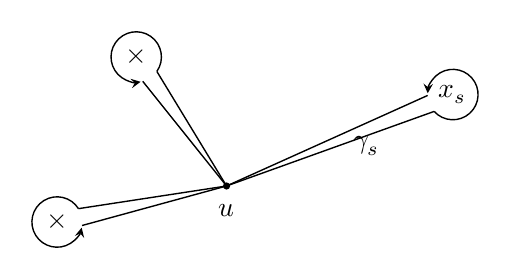
\begin{tikzpicture}[line width=0.5pt,>=stealth]
\coordinate (u) at (0,0);
\foreach \ang/\len/\lab in {125/2.0/{\times}, 192/2.2/{\times}, 22/3.1/{x_s}} {
  \coordinate (c) at (\ang:\len);
  \draw (u) -- ($(c)+(\ang+160:0.32)$);
  \draw (u) -- ($(c)+(\ang+200:0.32)$);
  \draw[->] ($(c)+(\ang+200:0.32)$) arc[start angle=\ang+200, end angle=\ang+515, radius=0.32];
  \node at (c) {$\lab$};
}
\fill (u) circle (1.3pt);
\node[below=3pt] at (u) {$u$};
\node at (16:1.85) {$\gamma_s$};
\end{tikzpicture}
\end{center}

\noindent The loops generate the fundamental group \(\pi _{1}(\mathrm{U},u)\). It acts on \(\mathrm{H}^{i}(\mathrm{X}_{u},\mathbf{Z})\), the fiber at \(u\) of the local system \(\mathrm{R}^{i} f_{*}\underline{\mathbf{Z}}|\mathrm{U}\). By the local theory (4.1), each \(s\in \mathrm{S}\) gives a vanishing cycle \(\delta _{s}\in \mathrm{H}^{n}(\mathrm{X}_{u},\mathbf{Z})\); these cycles depend on the choice of the \(\gamma _{s}\). For \(i\ne n\), the action of \(\pi _{1}(\mathrm{U},u)\) on \(\mathrm{H}^{i}(\mathrm{X}_{u},\mathbf{Z})\) is trivial. For \(i=n\), we have\par

\begin{equation*}\begin{gathered}\gamma _{s} x = x \pm  (x,\delta _{s})\delta _{s}.\end{gathered}\tag{5.2.1}\end{equation*}

\noindent Let \(\mathrm{E}\) be the subspace of \(\mathrm{H}^{n}(\mathrm{X}_{u},\mathbf{Q})\) spanned by the \(\delta _{s}\) (the \emph{vanishing} part of the cohomology).\par

\noindent \emph{Proposition} \textbf{(5.3)}. — {\itshape \(\mathrm{E}\) is stable under the action of the monodromy group \(\pi _{1}(\mathrm{U},u)\). The orthogonal complement \(\mathrm{E}^{\perp }\) of \(\mathrm{E}\) (with respect to the intersection form \(\operatorname{Tr}(x\cup y))\) is the subspace of monodromy invariants in \(\mathrm{H}^{n}(\mathrm{X}_{u},\mathbf{Q})\).}\par

\noindent Since the \(\gamma _{s}\) generate the monodromy group, this follows immediately from (5.2.1).\par

\noindent \emph{Theorem} \textbf{(5.4)}. — {\itshape The vanishing cycles \(\pm \delta _{s}\) (considered up to sign) are conjugate under the action of \(\pi _{1}(\mathrm{U},u)\).}\par

\noindent Let \(\check{\mathrm{X}}\subset \check{\mathbf{P}}\) be the dual variety of \(\mathrm{X}\): it consists of the \(t\in \check{\mathbf{P}}\) for which \(\mathrm{H}_{t}\) is tangent to \(\mathrm{X}\), i.e. for which \(\mathrm{X}_{t}\) is singular, or \(\mathrm{X}\subset \mathrm{H}_{t}\). The variety \(\check{\mathrm{X}}\) is irre-\par

\clearpage

\phantomsection\label{physical-20}

\noindent ducible. Let \(\mathrm{Y}\subset \mathrm{X}\times \check{\mathbf{P}}\) be the space of pairs (\(x,t)\) with \(x\in \mathrm{H}_{t}\). We have a diagram\par

\[\begin{array}{ccc}\mathrm X&\xleftarrow{}&\mathrm Y\\ &&\downarrow\!{g}\\ &&\check{\mathbf P}\end{array}\]

\noindent The fiber of \(g\) over \(t\in \check{\mathbf{P}}\) is the hyperplane section \(\mathrm{X}_{t}=\mathrm{X}\cap \mathrm{H}_{t}\) of \(\mathrm{X}\), and \(g\) is smooth away from the inverse image of \(\check{\mathrm{X}}\).\par

\noindent The setting of (5.1) is recovered by replacing \(\check{\mathbf{P}}\) with a line \(\mathrm{D}\subset \check{\mathbf{P}}\) and \(\mathrm{Y}\) with \(g^{- 1}(\mathrm{D})\). We have \(\mathrm{S}=\mathrm{D}\cap \check{\mathrm{X}}\). A theorem of Lefschetz asserts that, for \(\mathrm{D}\) sufficiently general, the map\par

\begin{equation*}\begin{gathered}\pi _{1}(\mathrm{D}- \mathrm{S},u) \longrightarrow  \pi _{1}(\check{\mathbf{P}}- \check{\mathrm{X}},u)\end{gathered}\end{equation*}

\noindent is surjective. Thus it suffices to prove that the \(\pm \delta _{s}\) are conjugate under \(\pi _{1}(\check{\mathbf{P}}- \check{\mathrm{X}})\).\par

\noindent For \(x\) in the smooth locus of codimension 1 of \(\check{\mathrm{X}}\), let \(ch\) be a path from \(t\) to \(x\) in \(\check{\mathbf{P}}- \check{\mathrm{X}}\), and \(\gamma _{x}\) the loop that follows \(ch\) up to a neighborhood of \(\check{\mathrm{X}}\), goes once around \(\check{\mathrm{X}}\), then returns to \(t\) along \(ch\). The loops \(\gamma _{x}\) (as \(ch\) varies) are all conjugate. Since \(\check{\mathrm{X}}\) is irreducible, two points in the smooth locus of \(\check{\mathrm{X}}\) can always be joined, within \(\check{\mathrm{X}}\), by a path that stays in the smooth locus. Consequently, the conjugacy class of \(\gamma _{x}\) is independent of \(x\). In particular, the \(\gamma _{s}\) are conjugate to one another. Formula (5.2.1) shows that the \(\pm \delta _{s}\) are therefore conjugate.\par

\noindent \emph{Corollary} \textbf{(5.5)}. — {\itshape The action of \(\pi _{1}(\mathrm{U},u)\) on \(\mathrm{E}/(\mathrm{E}\cap \mathrm{E}^{\perp })\) is absolutely irreducible.}\par

\noindent Let \(\mathrm{F}\subset \mathrm{E}\otimes \mathbf{C}\) be a monodromy-stable subspace. If \(\mathrm{F}\not\subset (\mathrm{E}\cap \mathrm{E}^{\perp })\otimes \mathbf{C}\), there are \(x\in \mathrm{F}\) and \(s\in \mathrm{S}\) such that (\(x,\delta _{s})\ne 0\). Then\par

\begin{equation*}\begin{gathered}\gamma _{s} x- x = \pm (x,\delta _{s})\delta _{s} \in  \mathrm{F},\end{gathered}\end{equation*}

\noindent and \(\delta _{s}\in \mathrm{F}\). By (5.4), all the \(\delta _{s}\) then lie in \(\mathrm{F}\), and  \(\mathrm{F}=\mathrm{E}\otimes \mathbf{C}\).  This proves (5.5).\par

\noindent \textbf{(5.6)} In abstract algebraic geometry these results take the following form.\par

\noindent Let \(\mathbf{P}\) be a projective space of dimension >1 over an algebraically closed field \(k\) of characteristic \(p\), and \(\mathrm{X}\subset \mathbf{P}\) a nonsingular connected projective variety of dimension \(n+1\). For a linear subspace \(\mathrm{A}\) of \(\mathbf{P}\) of codimension 2, we define D and the pencil (\(\mathrm{H}_{t})_{t\in \mathrm{D}}\), the \(\mathrm{X}_{t}, \widetilde{\mathrm{X}}\), and diagram (5.1.1) as in (5.1). We say that the (\(\mathrm{X}_{t})_{t\in \mathrm{D}}\) form a \emph{Lefschetz pencil} of hyperplane sections if the following conditions hold:\par

\noindent \(\mathrm{A})\) The axis \(\mathrm{A}\) meets \(\mathrm{X}\) transversely. The space \(\widetilde{\mathrm{X}}\) is then obtained from \(\mathrm{X}\) by blowing up \(\mathrm{A}\cap \mathrm{X}\), and is smooth.\par

\clearpage

\phantomsection\label{physical-21}

\noindent \(\mathrm{B})\) One can find a finite subset \(\mathrm{S}\) of \(\mathrm{D}\) and, for every \(s\in \mathrm{S}\), a point \(x_{s}\in \mathrm{X}_{s}\) such that \(f\) is smooth away from the \(x_{s}\).\par

\noindent C) \(x_{s}\) is an ordinary quadratic singular point of \(\mathrm{X}_{s}\).\par

\noindent For each \(s\in \mathrm{S}\), the local Lefschetz theory of § 4 applies to the spectrum \(\mathrm{D}_{s}\) of the henselization of the local ring of \(\mathrm{D}\) at \(s\), and to \(\widetilde{\mathrm{X}}_{\mathrm{D}_{s}}=\widetilde{\mathrm{X}}\times _{\mathrm{D}} \mathrm{D}_{s}\).\par

\noindent \textbf{(5.7)} Let \(\mathrm{N}\) be the dimension of \(\mathbf{P}, r\) an integer \(\geq 1\), and \(\iota _{(r)}\) the embedding of \(\mathbf{P}\) into projective space of dimension \(\binom{\mathrm{N}+r}{\mathrm{N}}- 1\), with homogeneous coordinates the monomials of degree \(r\) in the homogeneous coordinates of \(\mathbf{P}\). The hyperplane sections of \(\iota _{(r)}(\mathbf{P})\) are the hypersurfaces of degree \(r\) in \(\mathbf{P}\).\par

\noindent If \(p\ne 0\), it is possible that no pencil of hyperplane sections of \(\mathrm{X}\) is a Lefschetz pencil. However, if \(r\geq 2\) and the given projective embedding \(\iota _{1}:\mathrm{X}\hookrightarrow \mathbf{P}\) is replaced by \(\iota _{r}=\iota _{(r)}\circ \iota _{1}\), then, for this new embedding, every sufficiently general pencil is a Lefschetz pencil. In other words, if \(r\geq 2\), a sufficiently general pencil of hypersurface sections of degree \(r\) of \(\mathrm{X}\) is always a Lefschetz pencil.\par

\noindent \textbf{(5.8)} In the rest of this discussion we consider a Lefschetz pencil of hyperplane sections of \(\mathrm{X}\), \emph{excluding the case \(p=2, n\) even}. The case where \(n\) is odd would suffice for what follows. Set \(\mathrm{U}=\mathrm{D}- \mathrm{S}\). Let \(u\in \mathrm{U}\) and let \(\ell \) be a prime number \(\ne p\). The local results of § 4 show that \(\mathrm{R}^{n} f_{*}\mathbf{Q}_{\ell }\) is \emph{tamely} ramified at every \(s\in \mathrm{S}\). The tame fundamental group of \(\mathrm{U}\) is a quotient of the profinite completion of the analogous transcendental fundamental group (lifting tame coverings to characteristic 0, and the Riemann existence theorem). Thus the algebraic situation is just like the transcendental situation, and the results of Lefschetz carry over by standard arguments. In the proof of (5.4), the Lefschetz theorem on the \(\pi _{1}\) becomes Bertini's theorem, and we must invoke Abhyankar's lemma to control the ramification of \(\mathrm{R}^{\bullet} g_{*}\mathbf{Q}_{\ell }\) along the smooth locus of codimension one of \(\check{\mathrm{X}}\).\par

\noindent The results are the following.\par

\noindent a) \emph{If the vanishing cycles are nonzero:}\par

\noindent 1) For \(i\ne n\), the sheaf \(\mathrm{R}^{i} f_{*}\mathbf{Q}_{\ell }\) on \(\mathrm{D}\) is constant.\par

\noindent 2) Let \(j\) denote the inclusion of \(\mathrm{U}\) in \(\mathrm{D}\). We have\par

\begin{equation*}\begin{gathered}\mathrm{R}^{n} f_{*}\mathbf{Q}_{\ell } = j_{*}j^{*}\mathrm{R}^{n} f_{*}\mathbf{Q}_{\ell }.\end{gathered}\end{equation*}

\noindent 3) Let \(\mathrm{E}\subset \mathrm{H}^{n}(\mathrm{X}_{u},\mathbf{Q}_{\ell })\) be the subspace of cohomology spanned by the vanishing cycles. This subspace is stable under \(\pi _{1}(\mathrm{U},u)\), and\par

\begin{equation*}\begin{gathered}\mathrm{E}^{\perp } = \mathrm{H}^{n}(\mathrm{X}_{u},\mathbf{Q}_{\ell })^{\pi _{1}(\mathrm{U},u)}.\end{gathered}\end{equation*}

\noindent The representation of \(\pi _{1}(\mathrm{U},u)\) on \(\mathrm{E}/(\mathrm{E}\cap \mathrm{E}^{\perp })\) is absolutely irreducible, and the image of \(\pi _{1}\) in \(\operatorname{GL}(\mathrm{E}/(\mathrm{E}\cap \mathrm{E}^{\perp }))\) is generated (topologically) by the maps \(x\longrightarrow x\pm (x,\delta _{s})\delta _{s} (s\in \mathrm{S})\) (the sign \(\pm \) being determined as in (4.1)).\par

\clearpage

% ---- 03 ----
\phantomsection\label{physical-22}

\noindent b) \emph{If the vanishing cycles are zero:} (This is an exceptional case. Since (\(\delta ,\delta )=\pm 2\) for even \(n\), it can occur only for odd \(n\): \(n=2m+1\). Observe that if one vanishing cycle is zero, they are all zero, since they are conjugate.)\par

\noindent 1) For \(i\ne n+1\), the sheaf \(\mathrm{R}^{i} f_{*}\mathbf{Q}_{\ell }\) is constant.\par

\noindent 2) There is an exact sequence\par

\begin{equation*}\begin{gathered}0 \longrightarrow  \bigoplus\limits_{s\in \mathrm{S}} \mathbf{Q}_{\ell }(m- n)_{s} \longrightarrow  \mathrm{R}^{n+1}f_{*}\mathbf{Q}_{\ell } \longrightarrow  \mathcal{F}  \longrightarrow  0\end{gathered}\end{equation*}

\noindent with \(\mathcal{F} \) constant.\par

\noindent \(3) \mathrm{E}=0\).\par

\noindent \textbf{(5.9)} The subspace \(\mathrm{E}\cap \mathrm{E}^{\perp }\) of \(\mathrm{E}\) is the kernel of the restriction to \(\mathrm{E}\) of the intersection form \(\operatorname{Tr}(x\cup y)\). Thus this form induces a nondegenerate bilinear form\par

\begin{equation*}\begin{gathered}\psi  : \mathrm{E}/(\mathrm{E}\cap \mathrm{E}^{\perp })\otimes \mathrm{E}/(\mathrm{E}\cap \mathrm{E}^{\perp }) \longrightarrow  \mathbf{Q}_{\ell }(- n),\end{gathered}\end{equation*}

\noindent alternating when \(n\) is odd, and symmetric when \(n\) is even. Monodromy preserves this form; for odd \(n\), the monodromy representation therefore induces\par

\begin{equation*}\begin{gathered}\rho  : \pi _{1}(\mathrm{U},u) \longrightarrow  \operatorname{Sp}(\mathrm{E}/(\mathrm{E}\cap \mathrm{E}^{\perp }),\psi ).\end{gathered}\end{equation*}

\noindent \emph{Theorem} \textbf{(5.10)} (Kajdan-Margulis). — {\itshape \(\rho \) has open image.}\par

\noindent The image of \(\rho \) is a compact, and hence \(\ell \)-adic analytic, subgroup of \(\operatorname{Sp}(\mathrm{E}/(\mathrm{E}\cap \mathrm{E}^{\perp }),\psi )\). It is enough to prove that its Lie algebra \(\mathfrak{L} \) equals \(\mathfrak{sp}(\mathrm{E}/(\mathrm{E}\cap \mathrm{E}^{\perp }),\psi )\). In the transcendental setting, the analogue of this Lie algebra is the Lie algebra of the Zariski closure of the monodromy group.\par

\noindent From (5.8) it follows that \(\mathfrak{L} \) is generated by the square-zero transformations\par

\begin{equation*}\begin{gathered}\mathrm{N}_{s} : x \longmapsto  (x,\delta _{s})\delta _{s}    (s\in \mathrm{S})\end{gathered}\end{equation*}

\noindent and that \(\mathrm{E}/(\mathrm{E}\cap \mathrm{E}^{\perp })\) is an absolutely irreducible representation of \(\mathfrak{L} \). The following lemma yields the theorem.\par

\noindent \emph{Lemma} \textbf{(5.11)}. — {\itshape Let \(\mathrm{V}\) be a finite-dimensional vector space over a field \(k\) of characteristic \(0, \psi \) a nondegenerate alternating form and \(\mathfrak{L} \) a Lie subalgebra of \(\mathfrak{sp}(\mathrm{V},\psi )\). Assume that:}\par

\noindent {\itshape \textup{(i)} \(\mathrm{V}\) is a simple representation of \(\mathfrak{L} \).}\par

\noindent {\itshape \textup{(ii)} \(\mathfrak{L} \) is generated by a family of endomorphisms of \(\mathrm{V}\) of the form \(x\longmapsto \psi (x,\delta )\delta \).}\par

\noindent {\itshape Then \(\mathfrak{L} =\mathfrak{sp}(\mathrm{V},\psi )\).}\par

\noindent We may, and shall, assume that \(\mathrm{V}\), and hence \(\mathfrak{L} \), is nonzero. Let \(\mathrm{W}\subset \mathrm{V}\) be the set of \(\delta \in \mathrm{V}\) for which \(\mathrm{N}(\delta ):x\longmapsto \psi (x,\delta )\delta \) belongs to \(\mathfrak{L} \).\par

\noindent \emph{a)} \(\mathrm{W}\) is stable under homotheties (since \(\mathfrak{L} \) is a vector subspace of \(\mathfrak{gl}(\mathrm{V}))\).\par

\noindent \(b)\) If \(\delta \in \mathrm{W}, \operatorname{exp}(\lambda \mathrm{N}(\delta ))\) is an automorphism of (\(\mathrm{V},\psi ,\mathfrak{L} )\), and therefore maps \(\mathrm{W}\) to itself. If \(\delta ',\delta ''\in \mathrm{W}\), we therefore have \(\operatorname{exp}(\lambda \mathrm{N}(\delta '))\cdot \delta ''=\delta ''+\lambda \psi (\delta '',\delta ')\delta '\in \mathrm{W}\); if \(\psi (\delta ',\delta '')\ne 0\), the vector subspace spanned by \(\delta '\) and \(\delta ''\) is contained in \(\mathrm{W}\).\par

\clearpage

\phantomsection\label{physical-23}

\noindent \(c)\) Consequently, \(\mathrm{W}\) is the union of its maximal linear subspaces \(\mathrm{W}_{\alpha }\), and these are pairwise orthogonal. Each \(\mathrm{W}_{\alpha }\) is thus stable under the \(\mathrm{N}(\delta ) (\delta \in \mathrm{W})\), and hence under \(\mathfrak{L} \). In view of hypothesis (\(i), \mathrm{W}_{\alpha }=\mathrm{V}\) and \(\mathfrak{L} \) contains all the \(\mathrm{N}(\delta )\) for \(\delta \in \mathrm{V}\). We conclude by observing that the Lie algebra \(\mathfrak{sp}(\mathrm{V},\psi )\) is generated by the \(\mathrm{N}(\delta ) (\delta \in \mathrm{V})\).\par

\noindent \emph{Remark} \textbf{(5.12)} (not needed below). — It is now straightforward to prove (1.6) for a hypersurface of odd dimension \(n\) in \(\mathbf{P}^{n+1}_{\mathbf{F}_{q}}\).\par

\noindent Let \(\mathrm{X}_{0}\) be such a hypersurface, and \(\overline{\mathrm{X}}_{0}\) the hypersurface over \(\overline{\mathbf{F}}_{q}\) obtained from it by extension of scalars. We have\par

\begin{equation*}\begin{gathered}\mathrm{H}^{2i}(\overline{\mathrm{X}}_{0},\mathbf{Q}_{\ell })=\mathbf{Q}_{\ell }(- i)    (0\leq i\leq n);\end{gathered}\end{equation*}

\noindent \(\mathrm{H}^{2i}(\overline{\mathrm{X}}_{0},\mathbf{Q}_{\ell }(i))\) is generated by the \(i\)\textsuperscript{th} cup power of \(\eta \), the cohomology class \(c_{1}(\mathcal{O}(1))\) of a hyperplane section. We therefore have\par

\begin{equation*}\begin{gathered}\mathrm{Z}(\mathrm{X}_{0},t)=\operatorname{det}(1- \mathrm{F}^{*}t,\mathrm{H}^{n}(\overline{\mathrm{X}}_{0},\mathbf{Q}_{\ell })) / \prod _{i=0}^{n}(1- q^{i} t)\end{gathered}\end{equation*}

\noindent and \(\operatorname{det}(1- \mathrm{F}^{*}t,\mathrm{H}^{n}(\overline{\mathrm{X}}_{0},\mathbf{Q}_{\ell }))\) is a polynomial with integer coefficients independent of \(\ell \).\par

\noindent Let \(\mathrm{X}_{0}\) vary in a Lefschetz pencil of hypersurfaces defined over \(\mathbf{F}_{q}\) (cf. (5.7) for \(\mathrm{X}=\mathbf{P}^{n+1}\); the existence of such a pencil is not clear; to complete the argument sketched here, one would have to resort to the arguments to be given in (7.1)). One checks that \(\mathrm{E}\) here coincides with all of \(\mathrm{H}^{n}\), and (3.2) establishes the Weil conjecture for all the hypersurfaces in the pencil, in particular for \(\mathrm{X}_{0}\).\par

\noindent \textbf{(5.13)} \emph{Bibliographical references for §§ 4 and 5.}\par

\noindent \(\mathrm{A})\) Lefschetz’s results (4.1) and (5.1) through (5.5) are contained in his book [2]. For the local theory (4.1), consulting SGA 7, XIV (3.2) may be more convenient.\par

\noindent \(\mathrm{B})\) The results of § 4 are proved in Exposés XIII, XIV and XV of SGA 7.\par

\noindent C) (5.7) is proved in SGA 7, XVII.\par

\noindent D) (5.8) is proved in SGA 7, XVIII. The irreducibility theorem is proved there for \(\mathrm{E}\), but only under the assumption that \(\mathrm{E}\cap \mathrm{E}^{\perp }=\{0\}\). The proof in the general case (for \(\mathrm{E}/(\mathrm{E}\cap \mathrm{E}^{\perp }))\) is the same.\par

\section*{6. A rationality theorem.}

\noindent \textbf{(6.1)} Let \(\mathbf{P}_{0}\) be a projective space of dimension \(\geq 1\) over \(\mathbf{F}_{q}, \mathrm{X}_{0}\subset \mathbf{P}_{0}\) a nonsingular projective variety, \(\mathrm{A}_{0}\subset \mathbf{P}_{0}\) a linear subspace of codimension two, \(\mathrm{D}_{0}\subset \check{\mathbf{P}}_{0}\) the dual line, \(\overline{\mathbf{F}}_{q}\) an algebraic closure of \(\mathbf{F}_{q}\) and \(\mathbf{P}, \mathrm{X}, \mathrm{A}, \mathrm{D}\) over \(\overline{\mathbf{F}}_{q}\) obtained from \(\mathbf{P}_{0}, \mathrm{X}_{0}\),\par

\clearpage

\phantomsection\label{physical-24}\setcounter{page}{295}

\noindent \(\mathrm{A}_{0}, \mathrm{D}_{0}\) by extension of scalars. The diagram (5.1.1) in (5.6) arises from an analogous diagram over \(\mathbf{F}_{q}\):\par

\[\begin{array}{ccc}\mathrm X_0&\xleftarrow{\pi_0}&\widetilde{\mathrm X}_0\\ &&\downarrow\!{f_0}\\ &&\mathrm D_0\end{array}\tag{6.1.1}\]

\noindent Assume that \(\mathrm{X}\) is connected of \emph{even} dimension \(n+1=2m+2\), and that the pencil (\(\mathrm{X}_{t})_{t\in \mathrm{D}}\) of hyperplane sections of \(\mathrm{X}\) defined by \(\mathrm{D}\) is a \emph{Lefschetz pencil}. The set \(\mathrm{S}\) of \(t\in \mathrm{D}\) for which \(\mathrm{X}_{t}\) is singular is defined over \(\mathbf{F}_{q}\), i.e. comes from \(\mathrm{S}_{0}\subset \mathrm{D}_{0}\). Set \(\mathrm{U}_{0}=\mathrm{D}_{0}- \mathrm{S}_{0}\) and \(\mathrm{U}=\mathrm{D}- \mathrm{S}\).\par

\noindent Let \(u\in \mathrm{U}\). The vanishing part of the cohomology \(\mathrm{E}\subset \mathrm{H}^{n}(\mathrm{X}_{u},\mathbf{Q}_{\ell })\) is stable under \(\pi _{1}(\mathrm{U},u)\), and hence defines on \(\mathrm{U}\) a local subsystem \(\mathcal{E} \) of \(\mathrm{R}^{n} f_{*}\mathbf{Q}_{\ell }\). The latter is defined over \(\mathbf{F}_{q} : \mathrm{R}^{i} f_{*}\mathbf{Q}_{\ell }\) is the inverse image of the \(\mathbf{Q}_{\ell }\)-sheaf \(\mathrm{R}^{i} f_{0*}\mathbf{Q}_{\ell }\) on \(\mathrm{D}_{0}\), and, on \(\mathrm{U}, \mathcal{E} \) is the inverse image of a local subsystem\par

\begin{equation*}\begin{gathered}\mathcal{E} _{0} \subset  \mathrm{R}^{n} f_{0*}\mathbf{Q}_{\ell }.\end{gathered}\end{equation*}

\noindent The cup product is an alternating form\par

\begin{equation*}\begin{gathered}\psi  : \mathrm{R}^{n} f_{0*}\mathbf{Q}_{\ell }\otimes \mathrm{R}^{n} f_{0*}\mathbf{Q}_{\ell } \longrightarrow  \mathbf{Q}_{\ell }(- n).\end{gathered}\end{equation*}

\noindent Writing \(\mathcal{E} _{0}^{\perp }\) for the orthogonal complement of \(\mathcal{E} _{0}\) with respect to \(\psi \) in \(\mathrm{R}^{n} f_{0*}\mathbf{Q}_{\ell }|\mathrm{U}_{0}\), we see that \(\psi \) induces a perfect pairing\par

\begin{equation*}\begin{gathered}\psi  : \mathcal{E} _{0}/(\mathcal{E} _{0}\cap \mathcal{E} _{0}^{\perp })\otimes \mathcal{E} _{0}/(\mathcal{E} _{0}\cap \mathcal{E} _{0}^{\perp }) \longrightarrow  \mathbf{Q}_{\ell }(- n).\end{gathered}\end{equation*}

\noindent \emph{Theorem} \textbf{(6.2)}. — {\itshape For every \(x\in |\mathrm{U}_{0}|\), the polynomial \(\operatorname{det}(1- \mathrm{F}_{x}^{*}t,\mathcal{E} _{0}/(\mathcal{E} _{0}\cap \mathcal{E} _{0}^{\perp }))\) has rational coefficients.}\par

\noindent \emph{Corollary} \textbf{(6.3)}. — {\itshape Let \(j_{0}\) be the inclusion of \(\mathrm{U}_{0}\) into \(\mathrm{D}_{0}\), and \(j\) that of \(\mathrm{U}\) into \(\mathrm{D}\). The eigenvalues of \(\mathrm{F}^{*}\) acting on \(\mathrm{H}^{1}(\mathrm{D},j_{*}\mathcal{E} /(\mathcal{E} \cap \mathcal{E} ^{\perp }))\) are algebraic numbers whose complex conjugates \(\alpha \) all satisfy}\par

\begin{equation*}\begin{gathered}q^{\frac{n+1}{2}- \frac{1}{2}} \leq  |\alpha | \leq  q^{\frac{n+1}{2}+\frac{1}{2}}.\end{gathered}\end{equation*}

\noindent By (5.10) and (6.2), the hypotheses of (3.2) are indeed satisfied by (\(\mathrm{U}_{0},\mathcal{E} _{0}/(\mathcal{E} _{0}\cap \mathcal{E} _{0}^{\perp }),\psi )\), with \(\beta =n\), and we apply (3.9).\par

\noindent \emph{Lemma} \textbf{(6.4)}. — {\itshape Let \(\mathcal{G} _{0}\) be a locally constant \(\mathbf{Q}_{\ell }\)-sheaf on \(\mathrm{U}_{0}\), such that its inverse image \(\mathcal{G} \) on \(\mathrm{U}\) is a constant sheaf. There then exist in \(\overline{\mathbf{Q}}_{\ell }\) units \(\alpha _{i}\) such that, for every \(x\in |\mathrm{U}_{0}|\), we have}\par

\begin{equation*}\begin{gathered}\operatorname{det}(1- \mathrm{F}_{x}^{*}t,\mathcal{G} _{0})=\prod _{i}(1- \alpha _{i}^{\operatorname{deg}(x)}t).\end{gathered}\end{equation*}

\clearpage

\phantomsection\label{physical-25}\setcounter{page}{296}

\noindent This lemma says that \(\mathcal{G} _{0}\) is the inverse image of a sheaf on \(\operatorname{Spec}(\mathbf{F}_{q})\), namely its direct image on \(\operatorname{Spec}(\mathbf{F}_{q})\). The latter is identified with an \(\ell \)-adic representation \(\mathrm{G}_{0}\) of \(\operatorname{Gal}(\overline{\mathbf{F}}_{q}/\mathbf{F}_{q})\), and we take\par

\begin{equation*}\begin{gathered}\operatorname{det}(1- \mathrm{F}t,\mathrm{G}_{0})=\prod _{i}(1- \alpha _{i} t).\end{gathered}\end{equation*}

\noindent Lemma (6.4) applies to the \(\mathrm{R}^{i} f_{0*}\mathbf{Q}_{\ell } (i\ne n)\), to \(\mathrm{R}^{n} f_{0*}\mathbf{Q}_{\ell }/\mathcal{E} _{0}\) and to \(\mathcal{E} _{0}\cap \mathcal{E} _{0}^{\perp }\).\par

\noindent For \(x\in |\mathrm{U}_{0}|\), the fiber \(\mathrm{X}_{x}=f_{0}^{- 1}(x)\) is a variety over the finite field \(k(x)\). If \(\overline{x}\) is a point of \(\mathrm{U}\) lying over \(x, \mathrm{X}_{\overline{x}}\) is obtained from \(\mathrm{X}_{x}\) by extension of scalars from \(k(x)\) to its algebraic closure \(k(\overline{x})=\overline{\mathbf{F}}_{q}\), and \(\mathrm{H}^{i}(\mathrm{X}_{\overline{x}},\mathbf{Q}_{\ell })\) is the stalk of \(\mathrm{R}^{i} f_{*}\mathbf{Q}_{\ell }\) at \(\overline{x}\). Formula (1.5.4) for the variety \(\mathrm{X}_{x}\) over \(k(x)\) may thus be written\par

\begin{equation*}\begin{gathered}\mathrm{Z}(\mathrm{X}_{x},t)=\prod _{i} \operatorname{det}(1- \mathrm{F}_{x}^{*}t,\mathrm{R}^{i} f_{0*}\mathbf{Q}_{\ell })^{(- 1)^{i+1}}\end{gathered}\end{equation*}

\noindent and \(\mathrm{Z}(\mathrm{X}_{x},t)\) is the product of\par

\begin{equation*}\begin{gathered}\mathrm{Z}^{f}=\operatorname{det}(1- \mathrm{F}_{x}^{*}t,\mathrm{R}^{n} f_{0*}\mathbf{Q}_{\ell }/\mathcal{E} _{0})\cdot \operatorname{det}(1- \mathrm{F}_{x}^{*}t,\mathcal{E} _{0}\cap \mathcal{E} _{0}^{\perp })\cdot \prod _{i\ne n}\operatorname{det}(1- \mathrm{F}_{x}^{*}t,\mathrm{R}^{i} f_{0*}\mathbf{Q}_{\ell })^{(- 1)^{i+1}}\end{gathered}\end{equation*}

\noindent and\par

\begin{equation*}\begin{gathered}\mathrm{Z}^{m}=\operatorname{det}(1- \mathrm{F}_{x}^{*}t,\mathcal{E} _{0}/(\mathcal{E} _{0}\cap \mathcal{E} _{0}^{\perp })).\end{gathered}\end{equation*}

\noindent Set \(\mathcal{F} _{0}=\mathcal{E} _{0}/(\mathcal{E} _{0}\cap \mathcal{E} _{0}^{\perp }), \mathcal{F} =\mathcal{E} /(\mathcal{E} \cap \mathcal{E} ^{\perp })\) and apply (6.4) to the factors of \(\mathrm{Z}^{f}\). We find that there are \(\ell \)-adic units \(\alpha _{i} (1\leq i\leq \mathrm{N})\) and \(\beta _{j} (1\leq j\leq \mathrm{M})\) in \(\overline{\mathbf{Q}}_{\ell }\) such that for every \(x\in |\mathrm{U}_{0}|\)\par

\[\mathrm{Z}(\mathrm{X}_{x},t)=\frac{\prod\limits _{i}(1- \alpha _{i}^{\operatorname{deg} x}t)}{\prod\limits _{j}(1- \beta _{j}^{\operatorname{deg} x}t)}\cdot \operatorname{det}(1- \mathrm{F}_{x}^{*}t,\mathcal{F} _{0})\]

\noindent and in particular that the right-hand side belongs to \(\mathbf{Q}(t)\). If some \(\alpha _{i}\) coincides with some \(\beta _{j}\), we may simultaneously delete this \(\alpha _{i}\) from the \(\alpha \) list and this \(\beta _{j}\) from the \(\beta \) list. We may therefore, and shall, assume that \(\alpha _{i}\ne \beta _{j}\) for every \(i\) and every \(j\).\par

\noindent \textbf{(6.5)} It is enough to prove that the polynomials \(\prod _{i}(1- \alpha _{i} t)\) and \(\prod _{j}(1- \beta _{j} t)\) have rational coefficients, i.e. that the family of the \(\alpha _{i}\) (resp. the family of the \(\beta _{j})\) is defined over \(\mathbf{Q}\). We shall deduce this from the following propositions.\par

\noindent \emph{Proposition} \textbf{(6.6)}. — {\itshape Let (\(\gamma _{i}) (1\leq i\leq \mathrm{P})\) and (\(\delta _{j}) (1\leq j\leq \mathrm{Q})\) be two families of \(\ell \)-adic units in \(\overline{\mathbf{Q}}_{\ell }\). Assume that \(\gamma _{i}\ne \delta _{j}\). If \(\mathrm{K}\) is a sufficiently large finite set of integers \(\ne 1\), and \(\mathrm{L}\) a sufficiently large subset of density 0 of |\(\mathrm{U}_{0}|\), then, if \(x\in |\mathrm{U}_{0}|\) satisfies \(k\nmid \operatorname{deg}(x)\) (for every \(k\in \mathrm{K})\) and \(x\notin \mathrm{L}\), the denominator of}\par

\begin{equation*}\begin{gathered}\operatorname{det}(1- \mathrm{F}_{x}^{*}t,\mathcal{F} _{0})\prod _{i}(1- \gamma _{i}^{\operatorname{deg}(x)}t)/\prod _{j}(1- \delta _{j}^{\operatorname{deg}(x)}t),\end{gathered}\tag{6.6.1}\end{equation*}

\noindent {\itshape when written in lowest terms, is \(\prod _{j}(1- \delta _{j}^{\operatorname{deg}(x)}t)\).}\par

\noindent The proof will be given in (6.10-13). By (6.7) below, (6.6) yields\par

\clearpage

\phantomsection\label{physical-26}\setcounter{page}{297}

\noindent an intrinsic description of the family of the \(\delta _{j}\) in terms of the family of rational functions (6.6.1) for \(x\in |\mathrm{U}_{0}|\).\par

\noindent \emph{Lemma} \textbf{(6.7)}. — {\itshape Let \(\mathrm{K}\) be a finite set of integers \(\ne 1\) and (\(\delta _{j}) (1\leq j\leq \mathrm{Q})\) and (\(\varepsilon _{j}) (1\leq j\leq \mathrm{Q})\) two families of elements of a field. If, for every sufficiently large \(n\) not divisible by any of the \(k\in \mathrm{K}\), the family of the \(\delta _{j}^{n}\) agrees with that of the \(\varepsilon _{j}^{n}\) (up to order), then the family of the \(\delta _{j}\) agrees with that of the \(\varepsilon _{j}\) (up to order).}\par

\noindent We argue by induction on \(\mathrm{Q}\). The set of integers \(n\) such that \(\delta _{\mathrm{Q}}^{n}=\varepsilon _{j}^{n}\) is an ideal (\(n_{j})\). We shall show that there is a \(j_{0}\) with \(\delta _{\mathrm{Q}}=\varepsilon _{j_{0}}\). Otherwise, the \(n_{j}\) would be different from 1, and there would be arbitrarily large integers \(n\) divisible by none of the \(n_{j}\), nor by any of the \(k\in \mathrm{K}\). We would then have \(\delta _{\mathrm{Q}}^{n}\ne \varepsilon _{j}^{n}\), contrary to the hypothesis. Thus there is a \(j_{0}\) such that \(\delta _{\mathrm{Q}}=\varepsilon _{j_{0}}\). The conclusion follows upon applying the induction hypothesis to the families (\(\delta _{j}) (j\ne \mathrm{Q})\) and (\(\varepsilon _{j}) (j\ne j_{0})\).\par

\noindent \emph{Proposition} \textbf{(6.8)}. — {\itshape Let (\(\gamma _{i}) (1\leq i\leq \mathrm{P})\) and (\(\delta _{j}) (1\leq j\leq \mathrm{Q})\) be two families of \(\ell \)-adic units in \(\overline{\mathbf{Q}}_{\ell }, \mathrm{R}(t)=\prod _{i}(1- \gamma _{i} t)\) and \(\mathrm{S}(t)=\prod _{j}(1- \delta _{j} t)\). Suppose that for every \(x\in |\mathrm{U}_{0}|\),}\par

\begin{equation*}\begin{gathered}\prod _{i}(1- \delta _{i}^{\operatorname{deg}(x)}t)\text{ divides }\prod _{i}(1- \gamma _{i}^{\operatorname{deg}(x)}t)\cdot \operatorname{det}(1- \mathrm{F}_{x}^{*}t,\mathcal{F} _{0}).\end{gathered}\end{equation*}

\noindent {\itshape Then \(\mathrm{S}(t)\) divides \(\mathrm{R}(t)\).}\par

\noindent Remove pairs of common elements from the families (\(\gamma _{i})\) and (\(\delta _{j})\) until the hypothesis of (6.6) holds. Apply (6.6). By assumption, the rational functions (6.6.1) are polynomials. Thus no \(\delta \) remains, which means that \(\mathrm{S}(t)\) divides \(\mathrm{R}(t)\).\par

\noindent This proposition gives an intrinsic characterization of \(\mathrm{R}(t)\) in terms of the family of polynomials\par

\begin{equation*}\begin{gathered}\prod _{i}(1- \gamma _{i}^{\operatorname{deg}(x)}t)\cdot \operatorname{det}(1- \mathrm{F}_{x}^{*}t,\mathcal{F} _{0}).\end{gathered}\end{equation*}

\noindent It is the least common multiple of the polynomials \(\mathrm{S}(t)=\prod _{j}(1- \delta _{j} t)\) satisfying the hypothesis of (6.8).\par

\noindent \textbf{(6.9)} We prove (6.5) and hence (6.2) (modulo (6.6)). Take in (\(6.6) (\gamma _{i})=(\alpha _{i})\) and (\(\delta _{j})=(\beta _{j})\). This gives an intrinsic characterization of the family of the \(\beta _{j}\) in terms of the family of rational functions \(\mathrm{Z}(\mathrm{X}_{x},t) (x\in |\mathrm{U}_{0}|)\). Since these lie in \(\mathbf{Q}(t)\), the family of the \(\beta _{j}\) is defined over \(\mathbf{Q}\).\par

\noindent The polynomials \(\prod _{i}(1- \alpha _{i}^{\operatorname{deg}(x)}t)\cdot \operatorname{det}(1- \mathrm{F}_{x}^{*}t,\mathcal{F} _{0})\) therefore lie in \(\mathbf{Q}[t]\). Proposition (6.8) gives an intrinsic description of the family of the \(\alpha _{i}\) in terms of this family of polynomials. Hence the family of the \(\alpha _{i}\) is defined over \(\mathbf{Q}\).\par

\noindent \textbf{(6.10)} \emph{Preliminaries}. — Let \(u\in \mathrm{U}\) and let \(\mathcal{F} _{u}\) be the stalk of \(\mathcal{F} \) at \(u\). The arithmetic fundamental group \(\pi _{1}(\mathrm{U}_{0},u)\), an extension of \(\widehat{\mathbf{Z}}=\operatorname{Gal}(\overline{\mathbf{F}}_{q}/\mathbf{F}_{q})\) (generator: \(\varphi )\) by the geometric fundamental group \(\pi _{1}(\mathrm{U},u)\), acts on \(\mathcal{F} _{u}\) by symplectic similitudes:\par

\begin{equation*}\begin{gathered}\rho  : \pi _{1}(\mathrm{U}_{0},u) \longrightarrow  \operatorname{CSp}(\mathcal{F} _{u},\psi ).\end{gathered}\end{equation*}

\clearpage

\phantomsection\label{physical-27}\setcounter{page}{298}

\noindent We write \(\mu (g)\) for the multiplier of a symplectic similitude \(g\). Let\par

\begin{equation*}\begin{gathered}\mathrm{H}\subset \widehat{\mathbf{Z}}\times \operatorname{CSp}(\mathcal{F} _{u},\psi )\end{gathered}\end{equation*}

\noindent be the subgroup defined by the equation\par

\begin{equation*}\begin{gathered}q^{- n}=\mu (g)\end{gathered}\end{equation*}

\noindent (\(q\) being an \(\ell \)-adic unit, \(q^{n}\in \mathbf{Q}_{\ell }^{*}\) is defined for every \(n\in \widehat{\mathbf{Z}})\). That \(\psi \) takes values in \(\mathbf{Q}_{\ell }(- n)\) means that the map from \(\pi _{1}\) to \(\widehat{\mathbf{Z}}\times \operatorname{CSp}\), with components the canonical projection onto \(\widehat{\mathbf{Z}}\) and \(\rho \), factors through\par

\begin{equation*}\begin{gathered}\rho _{1} : \pi _{1}(\mathrm{U}_{0},u) \longrightarrow  \mathrm{H}.\end{gathered}\end{equation*}

\noindent \emph{Lemma} \textbf{(6.11)}. — {\itshape The image \(\mathrm{H}_{1}\) of \(\rho _{1}\) is open in \(\mathrm{H}\).}\par

\noindent Indeed, \(\pi _{1}(\mathrm{U}_{0},u)\) maps onto \(\widehat{\mathbf{Z}}\), and the image of \(\pi _{1}(\mathrm{U},u)=\operatorname{Ker}(\pi _{1}(\mathrm{U}_{0},u)\longrightarrow \widehat{\mathbf{Z}})\) in \(\operatorname{Sp}(\mathcal{F} _{u},\psi )=\operatorname{Ker}(\mathrm{H}\longrightarrow \widehat{\mathbf{Z}})\) is open (5.10).\par

\noindent \emph{Lemma} \textbf{(6.12)}. — {\itshape For \(\delta \in \overline{\mathbf{Q}}_{\ell }\) an \(\ell \)-adic unit, the set \(\mathrm{Z}\) of (\(n,g)\in \mathrm{H}_{1}\) for which \(\delta ^{n}\) is an eigenvalue of \(g\) is closed and has measure zero.}\par

\noindent Clearly, \(\mathrm{Z}\) is closed. For each \(n\in \widehat{\mathbf{Z}}\), let \(\operatorname{CSp}_{n}\) be the set of \(g\in \operatorname{CSp}(\mathcal{F} _{u},\psi )\) such that \(\mu (g)=q^{- n}\), and let \(\mathrm{Z}_{n}\) be the set of \(g\in \operatorname{CSp}_{n}\) such that \(\delta ^{n}\) is an eigenvalue of \(g\). Then \(\operatorname{CSp}_{n}\) is a homogeneous space under \(\operatorname{Sp}\), and one checks that \(\mathrm{Z}_{n}\) is a proper algebraic subspace of it, hence of measure 0. By (\(6.11), \mathrm{H}_{1}\cap (\{n\}\times \mathrm{Z}_{n})\) therefore has measure 0 in the inverse image in \(\mathrm{H}_{1}\) of \(n\), and we apply Fubini to the projection \(\mathrm{H}_{1}\longrightarrow \widehat{\mathbf{Z}}\).\par

\noindent \textbf{(6.13)} We prove (6.6). For each \(i\) and \(j\), the set of integers \(n\) such that \(\gamma _{i}^{n}=\delta _{j}^{n}\) consists of the multiples of a fixed integer \(n_{ij}\) (we do not exclude \(n_{ij}=0)\). By hypothesis, \(n_{ij}\ne 1\).\par

\noindent By (6.12) and the Čebotarev density theorem, the set of \(x\in |\mathrm{U}_{0}|\) such that some  \(\delta _{j}^{\operatorname{deg}(x)}\)  is an eigenvalue of \(\mathrm{F}_{x}^{*}\) acting on \(\mathcal{F} _{0}\) has density 0. For \(\mathrm{K}\) take the set of the \(n_{ij}\), and for \(\mathrm{L}\) the set of \(x\) just described.\par

\section*{7. End of the proof of 1.7.}

\noindent \emph{Lemma} \textbf{(7.1)}. — {\itshape Let \(\mathrm{X}_{0}\) be a nonsingular absolutely irreducible projective variety of \textup{even} dimension \(d\) over \(\mathbf{F}_{q}\). Let \(\mathrm{X}\) over \(\overline{\mathbf{F}}_{q}\) be obtained from \(\mathrm{X}_{0}\) by extension of scalars and let \(\alpha \) be an eigenvalue of \(\mathrm{F}^{*}\) acting on \(\mathrm{H}^{d}(\mathrm{X},\mathbf{Q}_{\ell })\). Then \(\alpha \) is an algebraic number whose complex conjugates, still denoted \(\alpha \), all satisfy}\par

\begin{equation*}\begin{gathered}q^{\frac{d}{2}- \frac{1}{2}} \leq  |\alpha | \leq  q^{\frac{d}{2}+\frac{1}{2}}.\end{gathered}\tag{7.1.1}\end{equation*}

\noindent We use induction on \(d\) (always assumed even). The case \(d=0\) is trivial, even without assuming \(\mathrm{X}_{0}\) absolutely irreducible; from now on we assume \(d\geq 2\). Set \(d=n+1=2m+2\).\par

\clearpage

\phantomsection\label{physical-28}\setcounter{page}{299}

\noindent If \(\mathbf{F}_{q'}\) is an extension of degree \(r\) of \(\mathbf{F}_{q}\) and \(\mathrm{X}'_{0}/\mathbf{F}_{q'}\) is obtained from \(\mathrm{X}_{0}/\mathbf{F}_{q}\) by extension of scalars, assertion (7.1) for \(\mathrm{X}_{0}/\mathbf{F}_{q}\) is equivalent to (7.1) for \(\mathrm{X}'_{0}/\mathbf{F}_{q'}\): just as \(q\) is replaced by \(q^{r}\), the eigenvalues of \(\mathrm{F}^{*}\) are replaced by their \(r\)\textsuperscript{th} powers.\par

\noindent By (5.7), under a suitable projective embedding \(i:\mathrm{X}\longrightarrow \mathbf{P}, \mathrm{X}\) admits a Lefschetz pencil of hyperplane sections. The preceding remark allows us to assume that \(i\) and this pencil are defined over \(\mathbf{F}_{q}\) (on replacing \(\mathbf{F}_{q}\) by a finite extension if necessary).\par

\noindent Suppose therefore that over \(\mathbf{F}_{q}\) there is a projective embedding \(\mathrm{X}_{0}\longrightarrow \mathbf{P}_{0}\) and a codimension-two subspace \(\mathrm{A}_{0}\) of \(\mathbf{P}_{0}\) defining a Lefschetz pencil. We use again the notation of (6.1) and (6.3). A further extension of scalars allows us to assume that:\par

\noindent \(a)\) The points of \(\mathrm{S}\) are defined over \(\mathbf{F}_{q}\).\par

\noindent \(b)\) The vanishing cycles at \(x_{s} (s\in \mathrm{S})\) are defined over \(\mathbf{F}_{q}\) (since only \(\pm \delta \) is intrinsic, they might be defined only over a quadratic extension).\par

\noindent \(c)\) There is a rational point \(u_{0}\in \mathrm{U}_{0}\). We take the corresponding point \(u\) of \(\mathrm{U}\) as base point.\par

\noindent \(d) \mathrm{X}_{u_{0}}=f_{0}^{- 1}(u_{0})\) admits a smooth hyperplane section \(\mathrm{Y}_{0}\), defined over \(\mathbf{F}_{q}\). Set \(\mathrm{Y}=\mathrm{Y}_{0}\otimes _{\mathbf{F}_{q}}\overline{\mathbf{F}}_{q}\).\par

\noindent Since \(\widetilde{\mathrm{X}}\) is obtained from \(\mathrm{X}\) by blowing up the smooth subvariety \(\mathrm{A}\cap \mathrm{X}\) of codimension two, we have\par

\begin{equation*}\begin{gathered}\mathrm{H}^{i}(\mathrm{X},\mathbf{Q}_{\ell }) \hookrightarrow  \mathrm{H}^{i}(\widetilde{\mathrm{X}},\mathbf{Q}_{\ell })\end{gathered}\end{equation*}

\noindent (in fact, \(\mathrm{H}^{i}(\widetilde{\mathrm{X}},\mathbf{Q}_{\ell })=\mathrm{H}^{i}(\mathrm{X},\mathbf{Q}_{\ell })\oplus \mathrm{H}^{i- 2}(\mathrm{A}\cap \mathrm{X},\mathbf{Q}_{\ell })(- 1))\). It therefore suffices to establish (7.1.1) for the eigenvalues \(\alpha \) of \(\mathrm{F}^{*}\) acting on \(\mathrm{H}^{d}(\widetilde{\mathrm{X}},\mathbf{Q}_{\ell })\).\par

\noindent The Leray spectral sequence for \(f\) takes the form\par

\begin{equation*}\begin{gathered}\mathrm{E}_{2}^{pq}=\mathrm{H}^{p}(\mathrm{D},\mathrm{R}^{q} f_{*}\mathbf{Q}_{\ell }) \Rightarrow  \mathrm{H}^{p+q}(\widetilde{\mathrm{X}},\mathbf{Q}_{\ell }).\end{gathered}\end{equation*}

\noindent We need only prove (7.1.1) for the eigenvalues \(\alpha \) of \(\mathrm{F}^{*}\) acting on the \(\mathrm{E}_{2}^{pq}\) for \(p+q=d=n+1\). These are:\par

\noindent A) \(\mathrm{E}_{2}^{2,n- 1}\). By (\(5.8), \mathrm{R}^{n- 1}f_{*}\mathbf{Q}_{\ell }\) is constant. By (2.10), we therefore have\par

\begin{equation*}\begin{gathered}\mathrm{E}_{2}^{2,n- 1}=\mathrm{H}^{n- 1}(\mathrm{X}_{u},\mathbf{Q}_{\ell })(- 1).\end{gathered}\end{equation*}

\noindent By the weak Lefschetz theorem (a corollary of SGA 4, XIV (3.2), and of Poincaré duality, SGA 4, XVIII), we have\par

\begin{equation*}\begin{gathered}\mathrm{H}^{n- 1}(\mathrm{X}_{u},\mathbf{Q}_{\ell })(- 1) \hookrightarrow  \mathrm{H}^{n- 1}(\mathrm{Y},\mathbf{Q}_{\ell })(- 1),\end{gathered}\end{equation*}

\noindent and we apply the induction hypothesis to \(\mathrm{Y}_{0}\).\par

\noindent B) \(\mathrm{E}_{2}^{0,n+1}\). If the vanishing cycles are nonzero, \(\mathrm{R}^{n+1}f_{*}\mathbf{Q}_{\ell }\) is constant and\par

\begin{equation*}\begin{gathered}\mathrm{E}_{2}^{0,n+1}=\mathrm{H}^{n+1}(\mathrm{X}_{u},\mathbf{Q}_{\ell }).\end{gathered}\end{equation*}

\clearpage

\begingroup\setlength{\parskip}{.20em}\setlength{\abovedisplayskip}{4pt}\setlength{\belowdisplayskip}{4pt}\setlength{\abovedisplayshortskip}{2pt}\setlength{\belowdisplayshortskip}{2pt}

\phantomsection\label{physical-29}\setcounter{page}{300}

\noindent The Gysin map\par

\begin{equation*}\begin{gathered}\mathrm{H}^{n- 1}(\mathrm{Y},\mathbf{Q}_{\ell })(- 1) \longrightarrow  \mathrm{H}^{n+1}(\mathrm{X}_{u},\mathbf{Q}_{\ell })\end{gathered}\end{equation*}

\noindent is surjective (this argument is dual to \(\mathrm{A}))\), and we apply the induction hypothesis to \(\mathrm{Y}_{0}\).\par

\noindent If the vanishing cycles are zero, the exact sequence in (\(5.8) b)\) gives an exact sequence\par

\begin{equation*}\begin{gathered}\bigoplus\limits_{s\in \mathrm{S}}\mathbf{Q}_{\ell }(m- n) \longrightarrow  \mathrm{E}_{2}^{0,n+1} \longrightarrow  \mathrm{H}^{n+1}(\mathrm{X}_{u},\mathbf{Q}_{\ell }).\end{gathered}\end{equation*}

\noindent The eigenvalue of \(\mathrm{F}\) acting on \(\mathbf{Q}_{\ell }(m- n)\) is \(q^{d/2}\), and \(\mathrm{H}^{n+1}\) is dealt with as above.\par

\noindent C) \(\mathrm{E}_{2}^{1,n}\). If the “hard” Lefschetz theorem were available, we would know that \(\mathcal{E} \cap \mathcal{E} ^{\perp }\) is zero, and that \(\mathrm{R}^{n} f_{*}\mathbf{Q}_{\ell }\) is the direct sum of \(j_{*}\mathcal{E} \) and a constant sheaf. The \(\mathrm{H}^{1}\) of a constant sheaf on \(\mathbf{P}^{1}\) is zero, and it would be enough to apply (6.3).\par

\noindent Since we have not yet proved “hard” Lefschetz, we shall have to proceed by dévissage. If the vanishing cycles are zero, \(\mathrm{R}^{n} f_{*}\mathbf{Q}_{\ell }\) is constant ((\(5.8) b))\) and \(\mathrm{E}_{2}^{1,n}=0\). We may therefore, and shall, assume that the vanishing cycles are nonzero. Filter \(\mathrm{R}^{n} f_{*}\mathbf{Q}_{\ell }=j_{*}j^{*}\mathrm{R}^{n} f_{*}\mathbf{Q}_{\ell } (5.8)\) by the subsheaves \(j_{*}\mathcal{E} \) and \(j_{*}(\mathcal{E} \cap \mathcal{E} ^{\perp })\). If the vanishing cycles \(\delta \) do not belong to \(\mathcal{E} \cap \mathcal{E} ^{\perp }\), we have exact sequences:\par

\begin{equation*}\begin{gathered}0 \longrightarrow  j_{*}\mathcal{E}  \longrightarrow  \mathrm{R}^{n} f_{*}\mathbf{Q}_{\ell } \longrightarrow \text{ constant sheaf }\longrightarrow  0.\end{gathered}\tag{7.1.2}\end{equation*}

\begin{equation*}\begin{gathered}0 \longrightarrow \text{ constant sheaf }j_{*}(\mathcal{E} \cap \mathcal{E} ^{\perp }) \longrightarrow  j_{*}\mathcal{E}  \longrightarrow  j_{*}(\mathcal{E} /(\mathcal{E} \cap \mathcal{E} ^{\perp })) \longrightarrow  0.\end{gathered}\tag{7.1.3}\end{equation*}

\noindent If, God forbid, the \(\delta \) belong to \(\mathcal{E} \cap \mathcal{E} ^{\perp }\), then \(\mathcal{E} \subset \mathcal{E} ^{\perp }\), and there are exact sequences:\par

\begin{equation*}\begin{gathered}0 \longrightarrow \text{ the constant sheaf }j_{*}\mathcal{E} ^{\perp } \longrightarrow  \mathrm{R}^{n} f_{*}\mathbf{Q}_{\ell } \longrightarrow \text{ a sheaf }\mathcal{F}  \longrightarrow  0\end{gathered}\tag{7.1.4}\end{equation*}

\begin{equation*}\begin{gathered}0 \longrightarrow  \mathcal{F}  \longrightarrow \text{ the constant sheaf }j_{*}j^{*}\mathcal{F}  \longrightarrow  \bigoplus\limits_{s\in \mathrm{S}}\mathbf{Q}_{\ell }(m- n)_{s} \longrightarrow  0.\end{gathered}\tag{7.1.5}\end{equation*}

\noindent In the first case, the long exact cohomology sequences give\par

\begin{equation*}\begin{gathered}\mathrm{H}^{1}(\mathrm{D},j_{*}\mathcal{E} ) \longrightarrow  \mathrm{H}^{1}(\mathrm{R}^{n} f_{*}\mathbf{Q}_{\ell }) \longrightarrow  0,\end{gathered}\tag{7.1.2′}\end{equation*}

\begin{equation*}\begin{gathered}0 \longrightarrow  \mathrm{H}^{1}(\mathrm{D},j_{*}\mathcal{E} ) \longrightarrow  \mathrm{H}^{1}(\mathrm{D},j_{*}(\mathcal{E} /(\mathcal{E} \cap \mathcal{E} ^{\perp })))\end{gathered}\tag{7.1.3′}\end{equation*}

\noindent and we apply (6.3).\par

\noindent In the second case, they give\par

\begin{equation*}\begin{gathered}0 \longrightarrow  \mathrm{H}^{1}(\mathrm{D},\mathrm{R}^{n} f_{*}\mathbf{Q}_{\ell }) \longrightarrow  \mathrm{H}^{1}(\mathrm{D},\mathcal{F} ),\end{gathered}\tag{7.1.4′}\end{equation*}

\begin{equation*}\begin{gathered}\bigoplus\limits_{s\in \mathrm{S}}\mathbf{Q}_{\ell }(m- n) \longrightarrow  \mathrm{H}^{1}(\mathrm{D},\mathcal{F} ) \longrightarrow  0\end{gathered}\tag{7.1.5′}\end{equation*}

\noindent and we observe that \(\mathrm{F}\) acts on  \(\mathbf{Q}_{\ell }(m- n)\)  by multiplication by \(q^{d/2}\).\par

\noindent \emph{Lemma} \textbf{(7.2)}. — {\itshape Let \(\mathrm{X}_{0}\) be a nonsingular absolutely irreducible projective variety of dimension \(d\) over \(\mathbf{F}_{q}\). Let \(\mathrm{X}\) over \(\overline{\mathbf{F}}_{q}\) be obtained from \(\mathrm{X}_{0}\) by extension of scalars and let \(\alpha \) be an eigenvalue of \(\mathrm{F}^{*}\) acting on \(\mathrm{H}^{d}(\mathrm{X},\mathbf{Q}_{\ell })\). Then \(\alpha \) is an algebraic number whose complex conjugates, still denoted \(\alpha \), all satisfy}\par

\begin{equation*}\begin{gathered}|\alpha |=q^{d/2}.\end{gathered}\end{equation*}

\clearpage

\endgroup

\phantomsection\label{physical-30}

\noindent Let us first prove that (\(7.2)\Rightarrow (1.7)\). For \(\mathrm{X}_{0}\) nonsingular and projective over \(\mathbf{F}_{q}\) and \(i\) an integer, we must prove the following assertion:\par

\noindent {\itshape \(\mathrm{W}(\mathrm{X}_{0,i})\). Let \(\mathrm{X}\) be obtained from \(\mathrm{X}_{0}\) by extension of scalars from \(\mathbf{F}_{q}\) to \(\overline{\mathbf{F}}_{q}\). If \(\alpha \) is an eigenvalue of \(\mathrm{F}^{*}\) acting on \(\mathrm{H}^{i}(\mathrm{X},\mathbf{Q}_{\ell })\), then \(\alpha \) is an algebraic number whose complex conjugates, still denoted \(\alpha \), all satisfy |\(\alpha |=q^{i/2}\).}\par

\noindent \(a)\) If \(\mathbf{F}_{q^{n}}\) is an extension of degree \(n\) of \(\mathbf{F}_{q}\), and \(\mathrm{X}'_{0}/\mathbf{F}_{q^{n}}\) is obtained from \(\mathrm{X}_{0}/\mathbf{F}_{q}\) by extension of scalars, then \(\mathrm{W}(\mathrm{X}_{0},i)\) is equivalent to \(\mathrm{W}(\mathrm{X}'_{0},i)\): extending scalars amounts to replacing \(\alpha \) by \(\alpha ^{n}\) and \(q\) by \(q^{n}\).\par

\noindent \(b)\) If \(\mathrm{X}_{0}\) is of pure dimension \(n, \mathrm{W}(\mathrm{X}_{0},i)\) is equivalent to \(\mathrm{W}(\mathrm{X}_{0},2n- i)\): this follows from Poincaré duality.\par

\noindent \(c)\) If \(\mathrm{X}_{0}\) is a disjoint union of varieties \(\mathrm{X}_{0}^{\alpha }, \mathrm{W}(\mathrm{X}_{0},i)\) is equivalent to the conjunction of the \(\mathrm{W}(\mathrm{X}_{0}^{\alpha },i)\).\par

\noindent \(d)\) If \(\mathrm{X}_{0}\) is of pure dimension \(n, \mathrm{Y}_{0}\) is a smooth hyperplane section of \(\mathrm{X}_{0}\), and \(i<n\), then \(\mathrm{W}(\mathrm{Y}_{0},i)\Rightarrow \mathrm{W}(\mathrm{X}_{0},i)\): this follows from the weak Lefschetz theorem.\par

\noindent To prove the assertions \(\mathrm{W}(\mathrm{X}_{0},i)\), we reduce successively:\par

\noindent — by \(c)\), to assuming that \(\mathrm{X}_{0}\) is of some pure dimension \(n\);\par

\noindent — by \(b)\), to assuming in addition that \(0\leq i\leq n\);\par

\noindent — by \(a)\) and \(d)\), to assuming in addition that \(i=n\);\par

\noindent — by \(a)\) and \(c)\), to assuming in addition that \(\mathrm{X}_{0}\) is absolutely irreducible.\par

\noindent This case is covered by (7.2).\par

\noindent \textbf{(7.3)} We prove (7.2). For every integer \(k, \alpha ^{k}\) is an eigenvalue of \(\mathrm{F}^{*}\) acting on \(\mathrm{H}^{kd}(\mathrm{X}^{k},\mathbf{Q}_{\ell })\) (Künneth formula). For even \(k\), (7.1) applies to \(\mathrm{X}^{k}\), giving\par

\begin{equation*}\begin{gathered}q^{\frac{kd}{2}- \frac{1}{2}} \leq  |\alpha ^{k}| \leq  q^{\frac{kd}{2}+\frac{1}{2}}\end{gathered}\end{equation*}

\noindent and\par

\begin{equation*}\begin{gathered}q^{\frac{d}{2}- \frac{1}{2k}} \leq  |\alpha | \leq  q^{\frac{d}{2}+\frac{1}{2k}}.\end{gathered}\end{equation*}

\noindent Letting \(k\) tend to infinity yields (7.2).\par

\section*{8. First applications.}

\noindent \emph{Theorem} \textbf{(8.1)}. — {\itshape Let \(\mathrm{X}_{0}\subset \mathbf{P}_{0}^{n+r}\) be a nonsingular complete intersection over \(\mathbf{F}_{q}\), of dimension \(n\) and multidegree (\(d_{1},\ldots ,d_{r})\). Let \(b'\) be the \(n^{\mathrm{th}}\) Betti number of nonsingular complex complete intersections of the same dimension and multidegree. Set \(b=b'\) for odd \(n\), and \(b=b'- 1\) for even \(n\). Then}\par

\begin{equation*}\begin{gathered}|\# \mathrm{X}_{0}(\mathbf{F}_{q})- \# \mathbf{P}^{n}(\mathbf{F}_{q})| \leq  b\cdot q^{n/2}.\end{gathered}\end{equation*}

\noindent Let \(\mathrm{X}/\overline{\mathbf{F}}_{q}\) be obtained from \(\mathrm{X}_{0}\), and let \(\mathbf{Q}_{\ell }\cdot \eta ^{i}\) be the line in \(\mathrm{H}^{2i}(\mathrm{X},\mathbf{Q}_{\ell })\) generated by the \(i^{\mathrm{th}}\) cup power of the cohomology class of a hyperplane section. On this line, \(\mathrm{F}^{*}\) acts by multiplication by \(q^{i}\). The cohomology of \(\mathrm{X}\) is the sum of the \(\mathbf{Q}_{\ell }\cdot \eta ^{i}\)\par

\clearpage

\phantomsection\label{physical-31}

\noindent (\(0 \leq  i \leq  n)\) and of the primitive part of \(\mathrm{H}^{n}(\mathrm{X}, \mathbf{Q}_{\ell })\), of dimension \(b\). By (1.5), there are thus \(b\) algebraic numbers \(\alpha _{j}\), the eigenvalues of \(\mathrm{F}^{*}\) acting on this primitive cohomology, such that\par

\begin{equation*}\begin{gathered}\# \mathrm{X}_{0}(\mathbf{F}_{q}) = \sum _{i=0}^{n} q^{i} + (-1)^{n} \sum _{j} \alpha _{j}.\end{gathered}\end{equation*}

\noindent By (\(1.7), |\alpha _{j}| = q^{n/2}\) and\par

\begin{equation*}\begin{gathered}|\# \mathrm{X}_{0}(\mathbf{F}_{q}) - \# \mathbf{P}^{n}(\mathbf{F}_{q})| = |\# \mathrm{X}_{0}(\mathbf{F}_{q}) - \sum _{i=0}^{n} q^{i}| = |\sum _{j} \alpha _{j}| \leq  \sum _{j} |\alpha _{j}| = b\cdot q^{n/2}.\end{gathered}\end{equation*}

\noindent \emph{Theorem} \textbf{(8.2)}. — {\itshape Let \(\mathrm{N}\) be an integer \(\geq  1, \varepsilon  : (\mathbf{Z}/\mathrm{N})^{*} \longrightarrow  \mathbf{C}^{*}\) a character, \(k\) an integer \(\geq  2\) and \(f\) a holomorphic modular form on \(\Gamma _{0}(\mathrm{N})\), of weight \(k\) and character \(\varepsilon  : f\) is a holomorphic function on the Poincaré upper half-plane \(\mathrm{X}\), such that for \(\begin{pmatrix}a&b\\c&d\end{pmatrix}\) \(\in  \operatorname{SL}(2, \mathbf{Z})\), with \(c \equiv  0 (\mathrm{N})\), we have}\par

\begin{equation*}\begin{gathered}f\left(\frac{az+b}{cz+d}\right) = \varepsilon (a)^{-1}(cz+d)^{k} f(z).\end{gathered}\end{equation*}

\noindent {\itshape Assume that \(f\) is \textup{cuspidal} and \textup{primitive} (“new” in the sense of Atkin-Lehner and Miyake), in particular an eigenvector of the Hecke operators \(\mathrm{T}_{p} (p \nmid  \mathrm{N})\). Set \(f = \sum _{n=1}^{\infty } a_{n} q^{n}\), with \(q = e^{2\pi iz}\) (and \(a_{1} = 1)\). Then, for a prime \(p\) not dividing \(\mathrm{N}\)}\par

\begin{equation*}\begin{gathered}|a_{p}| \leq  2\cdot p^{\frac{k-1}{2}}.\end{gathered}\end{equation*}

\noindent {\itshape In other words, the roots of the equation}\par

\begin{equation*}\begin{gathered}\mathrm{T}^{2} - a_{p} \mathrm{T} + \varepsilon (p)\cdot p^{k-1}\end{gathered}\end{equation*}

\noindent {\itshape have absolute value \(p^{\frac{k-1}{2}}\).}\par

\noindent In fact, these roots occur as eigenvalues of Frobenius acting on the \(\mathrm{H}^{k-1}\) of a nonsingular projective variety of dimension \(k-1\) defined over \(\mathbf{F}_{p}\).\par

\noindent Under restrictive hypotheses, this fact is proved in my Bourbaki talk (Modular forms and \(\ell \)-adic representations, talk 355, February 1969, in: \emph{Lecture Notes in Mathematics}, 179). The general case is not much harder.\par

\noindent \emph{Remark} \textbf{(8.3)}. — J. P. Serre and I have recently proved that (8.2) remains true for \(k = 1\). The proof is entirely different.\par

\noindent The following application was suggested to me by \(\mathrm{E}\). Bombieri.\par

\noindent \emph{Theorem} \textbf{(8.4)}. — {\itshape Let \(\mathrm{Q}\) be a polynomial in \(n\) variables and of degree \(d\) over \(\mathbf{F}_{q}, \mathrm{Q}_{d}\) the homogeneous part of degree \(d\) of \(\mathrm{Q}\) and \(\psi  : \mathbf{F}_{q} \longrightarrow  \mathbf{C}^{*}\) a nontrivial additive character on \(\mathbf{F}_{q}\). Assume that:}\par

\noindent {\itshape \textup{(i)} \(d\) is prime to \(p\);\\ \textup{(ii)} the hypersurface \(\mathrm{H}_{0}\) in \(\mathbf{P}^{n-1}_{\mathbf{F}_{q}}\) defined by \(\mathrm{Q}_{d}\) is smooth.}\par

\clearpage

% ---- 04 ----
\phantomsection\label{physical-32}

\noindent {\itshape Then}\par

\begin{equation*}\begin{gathered}|\sum _{x_{1},\ldots ,x_{n} \in  \mathbf{F}_{q}} \psi (\mathrm{Q}(x_{1},\ldots ,x_{n}))| \leq  (d-1)^{n} q^{n/2}.\end{gathered}\end{equation*}

\noindent By replacing \(\mathrm{Q}\) by a scalar multiple if necessary, we may assume (and shall assume) that\par

\begin{equation*}\begin{gathered}\psi (x) = \operatorname{exp}(2\pi i \operatorname{Tr}_{\mathbf{F}_{q}/\mathbf{F}_{p}}(x)/p).\end{gathered}\tag{8.4.1}\end{equation*}

\noindent Let \(\mathrm{X}_{0}\) be the étale covering of the affine space \(\mathrm{A}_{0}\) of dimension \(n\) over \(\mathbf{F}_{q}\) defined by the equation \(\mathrm{T}^{p} - \mathrm{T} = \mathrm{Q}\), and let \(\sigma \) denote the projection from \(\mathrm{X}_{0}\) to \(\mathrm{A}_{0}\) :\par

\begin{equation*}\begin{gathered}\sigma  : \mathrm{X}_{0} \longrightarrow  \mathrm{A}_{0}\end{gathered}\end{equation*}

\begin{equation*}\begin{gathered}\mathrm{X}_{0} = \operatorname{Spec}(\mathbf{F}_{q}[x_{1},\ldots ,x_{n},\mathrm{T}]/(\mathrm{T}^{p}-\mathrm{T}-\mathrm{Q})).\end{gathered}\end{equation*}

\noindent The covering \(\mathrm{X}_{0}\) is Galois, with Galois group \(\mathbf{Z}/p; i \in  \mathbf{Z}/p = \mathbf{F}_{p}\) acts by \(\mathrm{T} \longmapsto  \mathrm{T}+i\).\par

\noindent For \(x \in  \mathrm{A}_{0}(\mathbf{F}_{q})\), let us calculate the Frobenius endomorphism of the fiber of \(\mathrm{X}_{0}/\mathrm{A}_{0}\) at \(x\). Put \(q = p^{f}\) and let \(\overline{\mathbf{F}}_{q}\) be an algebraic closure of \(\mathbf{F}_{q}\). For (\(x,\mathrm{T}) \in  \mathrm{X}_{0}(\overline{\mathbf{F}}_{q})\) over \(x\), we have \(\mathrm{F}((x,\mathrm{T})) = (x,\mathrm{T}^{q})\), and\par

\begin{equation*}\begin{gathered}\mathrm{T}^{q} = \mathrm{T} + \sum _{i=1}^{f} (\mathrm{T}^{p^{i}}-\mathrm{T}^{p^{i-1}}) = \mathrm{T} + \sum _{i} \mathrm{Q}(x)^{p^{i-1}} = \mathrm{T} + \operatorname{Tr}_{\mathbf{F}_{q}/\mathbf{F}_{p}}(\mathrm{Q}(x)).\end{gathered}\end{equation*}

\noindent This is the action of the Galois group element \(\operatorname{Tr}_{\mathbf{F}_{q}/\mathbf{F}_{p}}(\mathrm{Q}(x))\).\par

\noindent Let \(\mathrm{E}\) denote the field of the \(p^{\mathrm{th}}\) roots of unity and \(\lambda \) a finite place of \(\mathrm{E}\) prime to \(p\). We shall work with \(\lambda \)-adic cohomology. For \(j \in  \mathbf{Z}/p\), let \(\mathcal{F} _{j,0}\) be the rank-one \(\mathrm{E}_{\lambda }\)-local system on \(\mathrm{A}_{0}\) defined by \(\mathrm{X}_{0}\) and \(\psi (-jx) : \mathbf{Z}/p \longrightarrow  \mathrm{E}^{*} \longrightarrow  \mathrm{E}_{\lambda }^{*}\) : we have \(\iota  : \mathrm{X}_{0} \longrightarrow  \mathcal{F} _{j,0}\) with \(\iota (i*x) = \psi (-ji)\iota (x)\). We drop the 0 when denoting the objects obtained from \(\mathrm{A}_{0}, \mathrm{X}_{0}, \mathcal{F} _{j,0}\) by extension of scalars to \(\overline{\mathbf{F}}_{q}\). The trace formula (1.12.1) for \(\mathcal{F} _{1,0}\) takes the form\par

\begin{equation*}\begin{gathered}\sum _{x_{1},\ldots ,x_{n} \in  \mathbf{F}_{q}} \psi (\mathrm{Q}(x_{1},\ldots ,x_{n})) = \sum _{i} (-1)^{i} \operatorname{Tr}(\mathrm{F}^{*}, \mathrm{H}_{c}^{i}(\mathrm{A},\mathcal{F} _{1})).\end{gathered}\tag{8.4.2}\end{equation*}

\noindent We have \(\sigma _{*}\mathrm{E}_{\lambda } = \bigoplus\limits_{j} \mathcal{F} _{j}\), and thus\par

\begin{equation*}\begin{gathered}\mathrm{H}_{c}^{*}(\mathrm{X},\mathbf{Q}_{\ell }) \otimes _{\mathbf{Q}_{\ell }} \mathrm{E}_{\lambda } = \bigoplus\limits_{j} \mathrm{H}_{c}^{*}(\mathrm{A},\mathcal{F} _{j}).\end{gathered}\tag{8.4.3}\end{equation*}

\noindent For \(j = 0, \mathcal{F} _{j}\) is the constant sheaf \(\mathrm{E}_{\lambda }\); this summand corresponds to the inclusion, by pullback, of the cohomology of \(\mathrm{A}\) into that of \(\mathrm{X}\).\par

\noindent \emph{Lemma} \textbf{(8.5)}. — {\itshape \textup{(i)} For \(j \ne  0, \mathrm{H}_{c}^{i}(\mathrm{A},\mathcal{F} _{j})\) vanishes for \(i \ne  n\); for \(i = n\), this cohomology space is of dimension (\(d-1)^{n}\).}\par

\noindent {\itshape \textup{(ii)} For \(j \ne  0\), the cup product}\par

\begin{equation*}\begin{gathered}\mathrm{H}_{c}^{n}(\mathrm{A},\mathcal{F} _{j}) \otimes  \mathrm{H}_{c}^{n}(\mathrm{A},\mathcal{F} _{-j}) \longrightarrow  \mathrm{H}_{c}^{2n}(\mathrm{A},\mathrm{E}_{\lambda }) \xrightarrow{\operatorname{Tr}} \mathrm{E}_{\lambda }(-n)\end{gathered}\end{equation*}

\noindent {\itshape is a perfect pairing.}\par

\noindent {\itshape \textup{(iii)} \(\mathrm{X}_{0}\) is an open subset of a nonsingular projective variety \(\mathrm{Z}_{0}\).}\par

\clearpage

\phantomsection\label{physical-33}

\noindent Let us derive (8.4) from (8.5). Let \(j_{0} : \mathrm{X}_{0} \hookrightarrow  \mathrm{Z}_{0}\) and let \(j : \mathrm{X} \hookrightarrow  \mathrm{Z}\) be obtained by extending scalars to \(\overline{\mathbf{F}}_{q}\). In view of (\(8.4.2), (i)\), and (1.7) for \(\mathrm{Z}_{0}\), it is enough to establish the injectivity of\par

\begin{equation*}\begin{gathered}\mathrm{H}_{c}^{n}(\mathrm{A},\mathcal{F} _{1}) \xrightarrow{\sigma ^{*}} \mathrm{H}_{c}^{n}(\mathrm{X},\mathcal{F} _{1}) = \mathrm{H}_{c}^{n}(\mathrm{X},\mathrm{E}_{\lambda }) \xrightarrow{j_{!}} \mathrm{H}^{n}(\mathrm{Z},\mathrm{E}_{\lambda }).\end{gathered}\end{equation*}

\noindent Since we have \(\operatorname{Tr}(a \cup  b) = \frac{1}{p} \operatorname{Tr}(j_{!}\sigma ^{*}a \cup  j_{!}\sigma ^{*}b)\), this injectivity is a consequence of (ii).\par

\noindent \textbf{(8.6)} Let us prove (8.5) (iii). Let \(\mathrm{P}_{0}\) be the projective space over \(\mathbf{F}_{q}\) completing \(\mathrm{A}_{0}\) by adjoining a hyperplane at infinity \(\mathrm{P}_{0}^{\infty }\), let \(\mathrm{H}_{0} \subset  \mathrm{P}_{0}^{\infty }\) have equation \(\mathrm{Q}_{d} = 0\), and let \(\mathrm{Y}_{0}\) be the covering of \(\mathrm{P}_{0}\) given by the normalization of \(\mathrm{P}_{0}\) in \(\mathrm{X}_{0}\).\par

\[\begin{array}{ccccc}\mathrm X_0&\hookrightarrow&\mathrm Y_0&&\\ {\scriptstyle\sigma}\downarrow&&\downarrow&&\\ \mathrm A_0&\hookrightarrow&\mathrm P_0&\hookleftarrow\mathrm P_0^\infty&\hookleftarrow\mathrm H_0\end{array}\tag{8.6.1}\]

\noindent Let us examine \(\mathrm{Y}_{0}/\mathrm{P}_{0}\) near infinity, locally for the étale topology.\par

\noindent \emph{Lemma} \textbf{(8.7)}. — {\itshape \(\mathrm{Y}_{0}\) is smooth away from the inverse image of \(\mathrm{H}_{0}\).}\par

\noindent The divisor of the rational function \(\mathrm{Q}\) on \(\mathrm{P}_{0}\) is the sum of its finite part \(\operatorname{div}(\mathrm{Q})_{f}\) and \((-d)\) times the hyperplane at infinity. We have :\par

\begin{equation*}\begin{gathered}\operatorname{div}(\mathrm{Q}) = \operatorname{div}(\mathrm{Q})_{f} - d\mathrm{P}_{0}^{\infty } \\ \operatorname{div}(\mathrm{Q})_{f} \cap  \mathrm{P}_{0}^{\infty } = \mathrm{H}_{0}.\end{gathered}\tag{8.7.1}\end{equation*}

\noindent At finite distance, \(\mathrm{Y}_{0} = \mathrm{X}_{0}\) is étale over \(\mathrm{A}_{0}\), and therefore smooth. At infinity, but away from the inverse image of \(\mathrm{H}_{0}\), there are local coordinates (\(z_{1},\ldots ,z_{n})\) with \(\mathrm{Q} = z_{1}^{-d}\) (this uses the fact that (\(d,p) = 1)\). In these coordinates, \(\mathrm{Y}_{0}\) appears as the product of a curve with a smooth space (corresponding to the coordinates \(z_{2},\ldots ,z_{n})\). Normality then implies that it is smooth.\par

\noindent \emph{Lemma} \textbf{(8.8)}. — {\itshape In an étale neighborhood of a point over \(\mathrm{H}_{0}, \mathrm{Y}_{0}\) is smooth over a fixed normal singular surface.}\par

\noindent This time, local coordinates can be chosen such that \(\mathrm{Q} = z_{1}^{-d}z_{2}\). Indeed, smoothness of \(\mathrm{H}_{0}\) implies that \(\operatorname{div}(\mathrm{Q})_{f}\) is smooth near infinity and intersects \(\mathrm{P}_{0}^{\infty }\) transversely. This form does not depend on the point chosen and involves only two coordinates, which gives the assertion.\par

\noindent \textbf{(8.9)} It is known that the following procedure (due to Zariski) resolves the singularities of surfaces : one alternates normalization with blowing up the (reduced) singular locus. The operations in question commute with étale localization and with products with a smooth space. Thus Zariski's procedure also resolves the singularities of a space such as \(\mathrm{Y}_{0}\), which is smooth over a surface locally for the étale topology. The resolution of \(\mathrm{Y}_{0}\) thus obtained is the required \(\mathrm{Z}_{0}\).\par

\clearpage

\phantomsection\label{physical-34}

\noindent If \(\mathrm{T}\) is a curve on a surface \(\mathrm{S}\), containing its singular locus, and \(\mathrm{T}'\) is the inverse image of \(\mathrm{T}\) in the Zariski resolution \(\mathrm{S}'\) of \(\mathrm{S}\), it is known that repeatedly blowing up in \(\mathrm{S}'\) the (reduced) singular locus of (\(\mathrm{T}')_{\mathrm{red}}\) produces a surface \(\mathrm{S}''\) such that the reduced inverse image (\(\mathrm{T}'')_{\mathrm{red}}\) of \(\mathrm{T}\) in \(\mathrm{S}''\) is a divisor with normal crossings. Once again, the operations involved commute with étale localization and with products with a smooth space. Arguing as before, and noting that (\(\mathrm{Y}_{0}\), the locus at infinity) is locally smooth over a pair (\(\mathrm{S},\mathrm{T})\), we can even choose \(\mathrm{Z}_{0}\) so that \(\mathrm{Z}_{0}-\mathrm{X}_{0}\) is a divisor with normal crossings.\par

\noindent \textbf{(8.10)} Let us prove (\(8.5) (i)\), (ii). These are geometric assertions; we can therefore work from now on over \(\overline{\mathbf{F}}_{q}\). Let \(\mathrm{S}'\) be the affine space over \(\overline{\mathbf{F}}_{q}\) parametrizing polynomials in \(n\) variables of degree \(\leq  d\), and let \(\mathrm{S}\) be the open subset of \(\mathrm{S}'\) corresponding to polynomials whose homogeneous part of degree \(d\) has nonzero discriminant. We write \(\mathrm{Q}_{\mathrm{S}} \in  \mathrm{H}^{0}(\mathrm{S},\mathcal{O}_{\mathrm{S}}[x_{1},\ldots ,x_{n}])\) for the universal polynomial over \(\mathrm{S}\), and \(\mathrm{X}_{\mathrm{S}}\) for the étale Galois covering of \(\mathrm{A}_{\mathrm{S}} = \mathrm{A}^{n} \times  \mathrm{S}\) defined by the equation \(\mathrm{T}^{p}-\mathrm{T} = \mathrm{Q}_{\mathrm{S}}\), with Galois group \(\mathbf{Z}/p\). Let \(\mathrm{P}_{\mathrm{S}} = \mathrm{P}^{n} \times  \mathrm{S}\) be the projective space over \(\mathrm{S}\) completing \(\mathrm{A}_{\mathrm{S}}\), and let \(\mathrm{Y}_{\mathrm{S}}\) be the normalization of \(\mathrm{P}_{\mathrm{S}}\) in \(\mathrm{X}_{\mathrm{S}}\). Over \(\mathrm{S}\), we have a diagram analogous to (8.6.1).\par

\noindent The local-coordinate expressions for \(\mathrm{Q}\) given in (8.7) and (8.8) still hold in the present setting, with parameters, so that, locally for the étale topology on \(\mathrm{Y}_{\mathrm{S}}, \mathrm{Y}_{\mathrm{S}}/\mathrm{S}\) is isomorphic to the product of \(\mathrm{S}\) (which is smooth) with a fiber. The canonical method of resolution used in (8.9) gives a relative compactification \(\mathrm{Z}_{\mathrm{S}}/\mathrm{S}\) of \(\mathrm{X}_{\mathrm{S}}/\mathrm{S}\), with \(\mathrm{Z}_{\mathrm{S}}-\mathrm{X}_{\mathrm{S}}\) a divisor with relative normal crossings over \(\mathrm{S}\)\par

\[\begin{array}{ccc}\mathrm X_{\mathrm S}&\xhookrightarrow{u}&\mathrm Z_{\mathrm S}\\ \downarrow{\scriptstyle\sigma}&&\downarrow{\scriptstyle f}\\ \mathrm A_{\mathrm S}&\xrightarrow{a}&\mathrm S\end{array}\]

\noindent (\(f\) proper and smooth, \(u\) an open immersion, \(\mathrm{Z}_{\mathrm{S}}-\mathrm{X}_{\mathrm{S}}\) a divisor with relative normal crossings).\par

\noindent Let \(\mathcal{F} _{j,\mathrm{S}}\) be the \(\mathrm{E}_{\lambda }\)-sheaf on \(\mathrm{A}_{\mathrm{S}}\) obtained, as in (8.4), from \(\mathrm{X}_{\mathrm{S}}/\mathrm{A}_{\mathrm{S}}\). We have \(\sigma _{*}\mathrm{E}_{\lambda } = \bigoplus\limits_{j} \mathcal{F} _{j,\mathrm{S}}\), and hence\par

\begin{equation*}\begin{gathered}\mathrm{R}^{*}(fu)_{!}(\mathrm{E}_{\lambda }) = \bigoplus\limits_{j} \mathrm{R}^{*}a_{!}\mathcal{F} _{j,\mathrm{S}}.\end{gathered}\end{equation*}

\noindent The properties of \(\mathrm{Z}_{\mathrm{S}}\) guarantee that the \(\mathrm{R}^{i}(fu)_{!}\mathrm{E}_{\lambda } = \mathrm{R}^{i}f_{*}(u_{!}\mathrm{E}_{\lambda })\) are locally constant sheaves on \(\mathrm{S}\). It follows that the \(\mathrm{R}^{i}a_{!}\mathcal{F} _{j,\mathrm{S}}\) are locally constant as well. Since \(\mathrm{S}\) is connected, it is enough to prove (\(8.5) (i)\), (ii) for \emph{one} particular polynomial \(\mathrm{Q}\). We shall choose \(\mathrm{Q} = \sum _{i} x_{i}^{d}\). This polynomial satisfies the nonsingularity condition, since (\(d,p) = 1\). For this polynomial, the variables separate in the exponential sum in (8.4). This corresponds to the fact that \(\mathcal{F} _{j}\) is the tensor product of the pullbacks of\par
\fancypagestyle{signature305}{\fancyfoot[R]{\shortstack[r]{\textit{305}\\\textbf{39}}}}\thispagestyle{signature305}

\clearpage

\phantomsection\label{physical-35}\noindent{\footnotesize Authority physical page 35; printed 306}\par\smallskip

\noindent analogous sheaves \(\mathcal{F} _{j}^{1}\) on the one-dimensional factors \(\mathrm{A}^{1}\) of \(\mathrm{A} = \mathrm{A}^{n}\). By the Künneth formula\par

\begin{equation*}\begin{gathered}\mathrm{H}^{*}(\mathrm{A},\mathcal{F} _{j}) = \bigotimes \mathrm{H}^{*}(\mathrm{A}^{1},\mathcal{F} _{j}^{1}).\end{gathered}\end{equation*}

\noindent This reduces the proof of (\(8.5) (i)\), (ii) to the case \(n = 1\) with \(\mathrm{Q}\) equal to \(x^{d}\).\par

\noindent \textbf{(8.11)} Let us consider this particular case. The covering \(\mathrm{X}\) of \(\mathrm{A}\) is irreducible, hence for \(i = 0,2\)\par

\begin{equation*}\begin{gathered}\mathrm{H}_{c}^{i}(\mathrm{A},\mathrm{E}_{\lambda }) \xrightarrow{\sim } \mathrm{H}_{c}^{i}(\mathrm{X},\mathrm{E}_{\lambda }).\end{gathered}\end{equation*}

\noindent Thus, for \(i \ne  1\) and \(j \ne  0\), we have\par

\begin{equation*}\begin{gathered}\mathrm{H}_{c}^{i}(\mathrm{A},\mathcal{F} _{j}) = 0.\end{gathered}\end{equation*}

\noindent Assertion (ii) follows from (2.8) or (2.12), together with the equality \(u_{!}\mathcal{F} _{j} = u_{*}\mathcal{F} _{j}\). To prove (\(i)\), it remains to check that\par

\begin{equation*}\begin{gathered}\chi _{c}(\mathrm{A},\mathcal{F} _{j}) = 1-d.\end{gathered}\end{equation*}

\noindent By the Euler-Poincaré formula (see Bourbaki lecture 286 of February 1965, by \(\mathrm{M}\). Raynaud), this is equivalent to the following lemma.\par

\noindent \emph{Lemma} \textbf{(8.12)}. — {\itshape The Swan conductor of \(\mathcal{F} _{j}\) at infinity equals \(d\).}\par

\noindent This is equivalent to the following statement.\par

\noindent \emph{Lemma} \textbf{(8.13)}. — {\itshape Let \(k\) be a finite field of characteristic \(p, y \in  k[[x]]\) an element of valuation \(d\) prime to \(p, \mathrm{L}\) the extension of \(\mathrm{K} = k((x))\) generated by the roots of \(\mathrm{T}^{p}-\mathrm{T} = y^{-1}\), and \(\chi \) the following character of \(\operatorname{Gal}(\mathrm{L}/\mathrm{K})\) with values in \(\mathbf{Z}/p\) :}\par

\begin{equation*}\begin{gathered}\chi (\sigma ) = \sigma \mathrm{T}-\mathrm{T}.\end{gathered}\end{equation*}

\noindent {\itshape Then, \(\chi \) has conductor \(d+1\).}\par

\noindent Extending the residue field reduces us to the assumption that \(k\) is algebraically closed rather than finite, and we apply : J. P. Serre, On local fields with algebraically closed residue field, \emph{Bull. Soc. Math. France}, 89 (1961), p. 105-154, no. 4.4.\par

\section*{BIBLIOGRAPHY}

\noindent [\(1] \mathrm{A}\). \textsc{Grothendieck}, Lefschetz formula and rationality of \(\mathrm{L}\)-functions, \emph{Bourbaki Seminar}, \textbf{279}, December 1964 (Benjamin).\par

\noindent [\(2] \mathrm{S}\). \textsc{Lefschetz}, \emph{Analysis situs and algebraic geometry} (Gauthier-Villars), 1924. Reprinted in : \emph{Selected papers} (Chelsea Publ. Co.).\par

\noindent [\(3] \mathrm{R}. \mathrm{A}\). \textsc{Rankin}, Contributions to the theory of Ramanujan's function \(\tau (n)\) and similar arithmetical functions. II, \emph{Proc. Camb. Phil. Soc.}, \textbf{35} (1939), 351-372.\par

\clearpage

\phantomsection\label{physical-36}\noindent{\footnotesize Authority physical page 36; printed 307}\par\smallskip

\noindent [\(4] \mathrm{A}\). \textsc{Weil}, Numbers of solutions of equations in finite fields, \emph{Bull. Am. Math. Soc.}, \textbf{55} (1949), p. 497-508.\par

\noindent SGA, \emph{Bois-Marie Seminar on Algebraic Geometry} (IHES) :\par

\noindent SGA 4, Theory of topoi and étale cohomology of schemes (directed by \(\mathrm{M}\). \textsc{Artin}, \(\mathrm{A}\). \textsc{Grothendieck} and J.-L. \textsc{Verdier}), \emph{Lecture Notes in Math.}, 269, 270, 305.\par

\noindent SGA 5, \emph{l-adic cohomology and \(\mathrm{L}\)-functions}, distributed by the IHES.\par

\noindent SGA 7, Monodromy groups in algebraic geometry.\par

\noindent 1\textsuperscript{st} part : directed by \(\mathrm{A}\). \textsc{Grothendieck}, \emph{Lecture Notes in Math.}, 288.\par

\noindent 2\textsuperscript{nd} part : by \(\mathrm{P}\). \textsc{Deligne} and \(\mathrm{N}\). \textsc{Katz}, \emph{Lecture Notes in Math.}, 340.\par

\begin{flushright}\emph{Manuscript received 20 September 1973.}\end{flushright}

\clearpage

\end{document}